\documentclass[12pt]{article}
\usepackage[utf8]{vietnam}
\usepackage[vietnamese=nohyphenation]{hyphsubst}
\usepackage[vietnamese]{babel}
\usepackage[table,dvipsnames]{xcolor} % Required for row coloring
\usepackage{booktabs} % Required for nicer horizontal lines
\usepackage{ragged2e}
\usepackage{xcolor}
\usepackage{caption}
\usepackage{subcaption}
\usepackage{float}
\usepackage{amsmath,amssymb,amsfonts}
\usepackage{graphicx}
\usepackage{adjustbox}
\usepackage{multicol}
\usepackage[inline,shortlabels]{enumitem}
\usepackage{forest}
\usepackage{setspace}
\usepackage{longtable}
\usepackage{bm} 
\usepackage[inkscapelatex=false]{svg}
\usepackage{titling}
\usepackage{tabularx}
\usepackage{makecell} 
\usepackage[T1]{fontenc}
\usepackage{lmodern,mathrsfs}
% \usepackage[draft]{hyperref}
\usepackage{hyperref}
\usepackage{xparse}
\usepackage[most]{tcolorbox}

%  biblatex (thay cho IEEEtran.bst) ------------------------------------
\usepackage[
    backend=bibtex,
    style=ieee,
    maxnames=1,     % chỉ hiển thị 1 tên tác giả, phần còn lại thành "et al."
    minnames=1,
    uniquelist=false,
    hyperref=false
]{biblatex}

\addbibresource{references.bib}
\DefineBibliographyStrings{english}{
  andothers = {et\addabbrvspace al\adddot}
}
\AtBeginBibliography{\selectlanguage{english}}

% -----------------------------------------------------------------
\AtBeginDocument{\renewcommand\refname{}}

\usepackage[toc,page]{appendix}
\renewcommand{\appendixtocname}{Phụ lục}      
\renewcommand{\appendixpagename}{Phụ lục}

\usepackage{xurl}
\setlength{\headheight}{14.5pt}
\setlength{\topmargin}{-.5in} \setlength{\textheight}{9.25in}
\setlength{\oddsidemargin}{-0.1in} \setlength{\textwidth}{6.8in}

\usepackage{tocloft}
\renewcommand{\cfttoctitlefont}{\Huge\bfseries}
\setlength{\cftaftertoctitleskip}{2em}
\setlength{\cftbeforesubsecskip}{7pt} % giãn cách subitem mục lục
\renewcommand{\cftsecleader}{\cftdotfill{\cftdotsep}}
\setlength{\cftsecnumwidth}{3em}
\renewcommand{\cftsecaftersnum}{\quad}
\renewcommand{\cftsubsecleader}{\cftdotfill{\cftdotsep}}
\setlength{\cftsubsecnumwidth}{4em}
\renewcommand{\cftsubsecaftersnum}{\quad}
\renewcommand{\cftsubsubsecleader}{\cftdotfill{\cftdotsep}}
\setlength   {\cftsubsubsecnumwidth}{5em}  
\renewcommand{\cftsubsubsecaftersnum}{\quad}

\PassOptionsToPackage{vietnamese.licr}{babel}
\usepackage{vipythonhighlight} 
\newcounter{mycounter}
\newcommand\showmycounter{\stepcounter{mycounter}\themycounter}
\usepackage{lipsum}
\newcommand\showlips{\stepcounter{mycounter}\lipsum[\value{mycounter}]}

%--------------------------------------------------------------------
\usepackage{framed}
\usepackage{fancyhdr}

\usepackage{listings}	 % Sử dụng gói lệnh listings đề chèn code
\usepackage{tvietlistings}		    % Sử dụng Tiếng Việt trong gói listings

% Color --------------------------------------------------------------------
\usepackage{epigraph}
\usepackage{titlesec}

\definecolor{codebackground}{RGB}{250, 250, 250}
\definecolor{codecomment}{RGB}{34, 139, 34}
\definecolor{codekeyword}{RGB}{0, 0, 255}
\definecolor{codestring}{RGB}{255, 0, 0}
\definecolor{codeidentifier}{RGB}{0, 0, 0}
\definecolor{codelinenumbers}{RGB}{90, 90, 90}

\definecolor{codegreen}{rgb}{0,0.6,0}
\definecolor{codegray}{rgb}{0.5,0.5,0.5}
\definecolor{codepurple}{rgb}{0.58,0,0.82}
\definecolor{backcolour}{rgb}{0.95,0.95,0.92}

\definecolor{aivnGreen}{RGB}{52,79,30}  
\definecolor{captiongray}{gray}{0.15} 
\definecolor{captionbg}{RGB}{250,250,250}

% Table
\newtcolorbox{captionbelowboxaivn}{
    colback=aivnGreen,
    colframe=aivnGreen,
    boxrule=0pt,
    arc=4pt,
    left=4pt,
    right=4pt,
    top=2pt,
    bottom=2pt,
    width=\linewidth,
    boxsep=4pt,
    halign=center,
    % fontupper=\bfseries\color{white}
    fontupper=\color{white}
}

% Figure
\newtcolorbox{figurecardcaptionaivn}{
  colback=aivnGreen,        % Màu nền (background color)
  colframe=aivnGreen,       % Màu viền box (border color)
  boxrule=0pt,              % Độ dày viền box (0pt = không viền)
  arc=2pt,                  % Độ bo góc (2pt là bo nhẹ, tăng để bo tròn hơn)
  top=3pt,                  % Padding phía trên nội dung
  bottom=3pt,               % Padding phía dưới nội dung
  left=10pt,                % Padding bên trái
  right=10pt,               % Padding bên phải
  width=\linewidth,         % Chiều rộng bằng toàn bộ dòng
  fontupper=\small\fontsize{11pt}{13pt}\selectfont\color{white} 
}

% Tạo counter riêng
\newcounter{hinh}
% Định nghĩa macro caption Hình
\newcommand{\capfig}[1]{%
  \refstepcounter{hinh}%
  % \textbf{Hình~\thehinh:}~#1
    Hình~\thehinh:~#1
}

\newtcolorbox{figurecaptionmodern}{
  colback=captionbg,
  colframe=aivnGreen,
  boxrule=1.5pt,
  bottomrule=2pt,  
  toptitle=0pt,
  bottomtitle=0pt,
  left=6pt,
  right=6pt,
  top=4pt,
  bottom=2pt,
  width=\linewidth,
  fontupper=\small\fontsize{11pt}{13pt}\selectfont\color{black},
  halign=center
}

% Code Block -----------------------------------------------------------------
\newtcolorbox{aivncodebox}[1][]{%
  enhanced,
  colback=gray!10,
  colframe=aivnGreen,
  coltitle=white,
  colbacktitle=aivnGreen,
  title=#1,
  fonttitle=\bfseries\sffamily,
  listing only,
  breakable,
  listing engine=listings,
  listing options={
    language=Python,
    basicstyle=\ttfamily\footnotesize,
    commentstyle=\color{ForestGreen},
    keywordstyle=\color{blue},
    stringstyle=\color{red!70!black},
    numbers=left,
    numberstyle=\tiny\color{gray},
    numbersep=5pt,
    breaklines=true,
    showstringspaces=false,
    xleftmargin=1.5em,
    framexleftmargin=1.5em
  }
}

% Last argument allows more tcolorbox options to be added

%--------------------------------------------------------------------
\lstdefinestyle{mystyle}{
    backgroundcolor=\color{codebackground},
    commentstyle=\color{codecomment},
    keywordstyle=\color{codekeyword},
    stringstyle=\color{codestring},
    identifierstyle=\color{codeidentifier},
    basicstyle=\ttfamily\footnotesize,
    breakatwhitespace=false,
    breaklines=true,
    captionpos=b,
    keepspaces=true,
    numbers=left,
    numberstyle=\tiny\color{codelinenumbers}, 
    numbersep=5pt,
    showspaces=false,
    showstringspaces=false,
    showtabs=false,
    tabsize=2
}

\lstset{style=mystyle}

\hypersetup{
    colorlinks=true,
    linkcolor=black,
    filecolor=magenta,    
    citecolor=black,
    urlcolor=black,
    pdftitle={Overleaf Example},
    pdfpagemode=FullScreen,
}

%--------------------------------------------------------------------
\newcounter{choice}
\renewcommand\thechoice{($\alph{choice}$)}
\newcommand\choicelabel{\thechoice}

%--------------------------------------------------------------------
\newenvironment{choices}%
  {\list{\choicelabel}%
     {\usecounter{choice}\def\makelabel##1{\hss\llap{##1}}%
       \settowidth{\leftmargin}{W.\hskip\labelsep\hskip 0 em}%
       \def\choice{%
         \item
       } % choice
       \labelwidth\leftmargin\advance\labelwidth-\labelsep
       \topsep=0pt
       \partopsep=0pt
     }%
  }%
  {\endlist}
  
%--------------------------------------------------------------------
\def\CChoice{%
      \choice
      \addanswer{\theenumi}{\thechoice}%
    }
    \let\CChoice\CChoice
%    \par % Uncomment this to have choices always start a new line
   % \let\par\@empty
    % If we're continuing the paragraph containing the question,
    % then leave a bit of space before the first choice:
    \ifvmode\else\enskip\fi
    \ignorespaces
  %
  {}
\makeatother
\newbox\allanswers
\setbox\allanswers=\hbox{}
\newcommand{\addanswer}[2]{%
  \global\setbox\allanswers=\hbox{\unhbox\allanswers \quad #1.~#2}%
}
\newcommand{\showanswers}{%
  \vfill
  \begin{center}
    Answers
  \end{center}
  \unhbox\allanswers
}

\makeatletter
\newenvironment{multichoices}[1][1]{%
\begin{multicols}{#1}}{%
\end{multicols}}
\makeatother

\lstset{style=mystyle}
\pagestyle{fancy}

\DeclareMathOperator*{\argmax}{arg\,max}
\DeclareMathOperator*{\argmin}{arg\,min}
\DeclareMathOperator{\E}{\mathbb{E}}

% Outline --------------------------------------------------------------------
\renewcommand{\thesection}{\Roman{section}.} 
\renewcommand{\thesubsection}{\thesection\arabic{subsection}.}
\renewcommand{\thesubsubsection}{\thesubsection\arabic{subsubsection}.} 

\titleformat{\section}{\normalfont\Huge\bfseries}{\thesection}{1em}{}
\titleformat{\subsection}{\normalfont\Large\bfseries}{\thesubsection}{1em}{}
\titleformat{\subsubsection}{\normalfont\normalsize\bfseries}{\thesubsubsection}{1em}{}


% Logo --------------------------------------------------------------------
\setlength{\droptitle}{-8em}
\pretitle{%
    \begin{flushleft}
        \includegraphics[height=2.0cm]{Figures/logo.pdf}\par
    \end{flushleft}
}
\posttitle{}

% Title --------------------------------------------------------------------
\title{%
  \begin{center}
        \Large {AI VIET NAM -- AI COURSE 2025}\\[.5ex]  
        \Huge \textbf{Tutorial: Tableau}\\[.5ex]
  \end{center}
}

% Author --------------------------------------------------------------------
\posttitle{
    \author{
        \begin{minipage}{\textwidth}
        \centering
        {
          Thao-Nhi,\quad
          Anh-Nguyen
        }\\
      \end{minipage}
    }
}
% \setlength{\drop}{-8em}
\date{}

% Header --------------------------------------------------------------------
\pagestyle{fancy}
\fancyhf{}
\lhead{\href{https://www.facebook.com/aivietnam.edu.vn}{\textcolor{aivnGreen}{\bfseries AI VIET NAM (AIO2025)}}}
\rhead{\href{https://aivietnam.edu.vn/}{\textcolor{aivnGreen}{\bfseries aivietnam.edu.vn}}}
\fancyfoot[C]{\thepage}
\renewcommand{\headrulewidth}{1.0pt}
\renewcommand{\headrule}{{\color{aivnGreen}\hrule width\headwidth height\headrulewidth \vskip-\headrulewidth}}

% Document -------------------------------------------------------------------
\begin{document}
\maketitle
\vspace{-3.5em}

% ===================================================================
% PHẦN I & II — Thảo Nhi (để trống, điền sau)
% ===================================================================
\section{Giới thiệu}
\label{section:intro}

% TODO: Thảo Nhi — Giới thiệu Tableau, Visualization (Python, Tableau, Power BI), Demo dashboard mẫu
\textit{(Nội dung phần này sẽ được bổ sung sau — Thảo Nhi)}

\newpage
\setcounter{tocdepth}{2}
\tableofcontents
\thispagestyle{fancy}

\newpage
\section{Tableau UI \& Core Concepts}
\label{section:ui}

% TODO: Thảo Nhi — Interface overview, data pane, worksheet/dashboard, dimensions vs measures, rows, columns, marks card
\textit{(Nội dung phần này sẽ được bổ sung sau — Thảo Nhi)}


% ===================================================================
% PHẦN III — Preprocessing Functions (Anh Nguyên)
% ===================================================================
\newpage
\section{Preprocessing Functions trong Tableau (theo Data Type)}
\label{section:preprocessing}




\begin{conceptbox}{Dataset sử dụng trong ví dụ}
\textbf{Tableau Superstore} --- bộ dữ liệu mẫu có sẵn trong Tableau Desktop, tại menu \textbf{Help $\rightarrow$ Sample Workbooks $\rightarrow$ Superstore}. Dataset gồm $\sim$10.000 dòng đơn hàng bán lẻ với các trường về sản phẩm, khách hàng, doanh thu và lợi nhuận.
\end{conceptbox}


% ===================================================================
\subsection{Giới thiệu --- Dữ liệu thực tế không bao giờ ``sạch'' ngay từ đầu}
% ===================================================================

\noindent Trong thực tế, hầu hết các bộ dữ liệu đều mang theo những vấn đề tiềm ẩn mà mắt thường khó nhận ra. Một file CSV xuất từ hệ thống ERP có thể chứa tên khách hàng bị viết không nhất quán (\texttt{"nguyen van a"} và \texttt{"NGUYEN VAN A"} là hai khách hàng khác nhau trong mắt Tableau), cột ngày tháng bị lưu dưới dạng văn bản thay vì kiểu Date thực sự, hay cột doanh thu bị nhận nhầm là String khiến Tableau từ chối tính tổng.

\noindent Thông thường, các lỗi này được xử lý trong Python với Pandas trước khi đưa vào Tableau. Tuy nhiên, Tableau cung cấp một công cụ mạnh mẽ ngay bên trong môi trường phân tích --- \textbf{Calculated Field} --- cho phép chúng ta biến đổi, chuẩn hóa và tạo cột mới mà không cần rời khỏi Tableau. Điều này đặc biệt hữu ích khi dữ liệu nguồn cập nhật thường xuyên và ta không muốn phải chạy lại pipeline xử lý mỗi lần.

\begin{conceptbox}{Calculated Field (Trường tính toán)}
\textbf{Calculated Field} là một cột dữ liệu mới được tạo ra bằng cách viết biểu thức (expression) trực tiếp trong Tableau. Calculated Field không thay đổi dữ liệu gốc trong nguồn --- nó chỉ thực hiện phép tính tại thời điểm hiển thị, giống như một cột ``ảo'' được tính toán theo thời gian thực.

\noindent \textbf{Cách tạo:} Trên thanh menu, chọn \textbf{Analysis} $\rightarrow$ \textbf{Create Calculated Field...} Cửa sổ công thức sẽ hiện ra, nơi bạn nhập biểu thức và Tableau sẽ gợi ý hàm tự động.
\end{conceptbox}

\begin{figure}[H]
\centering
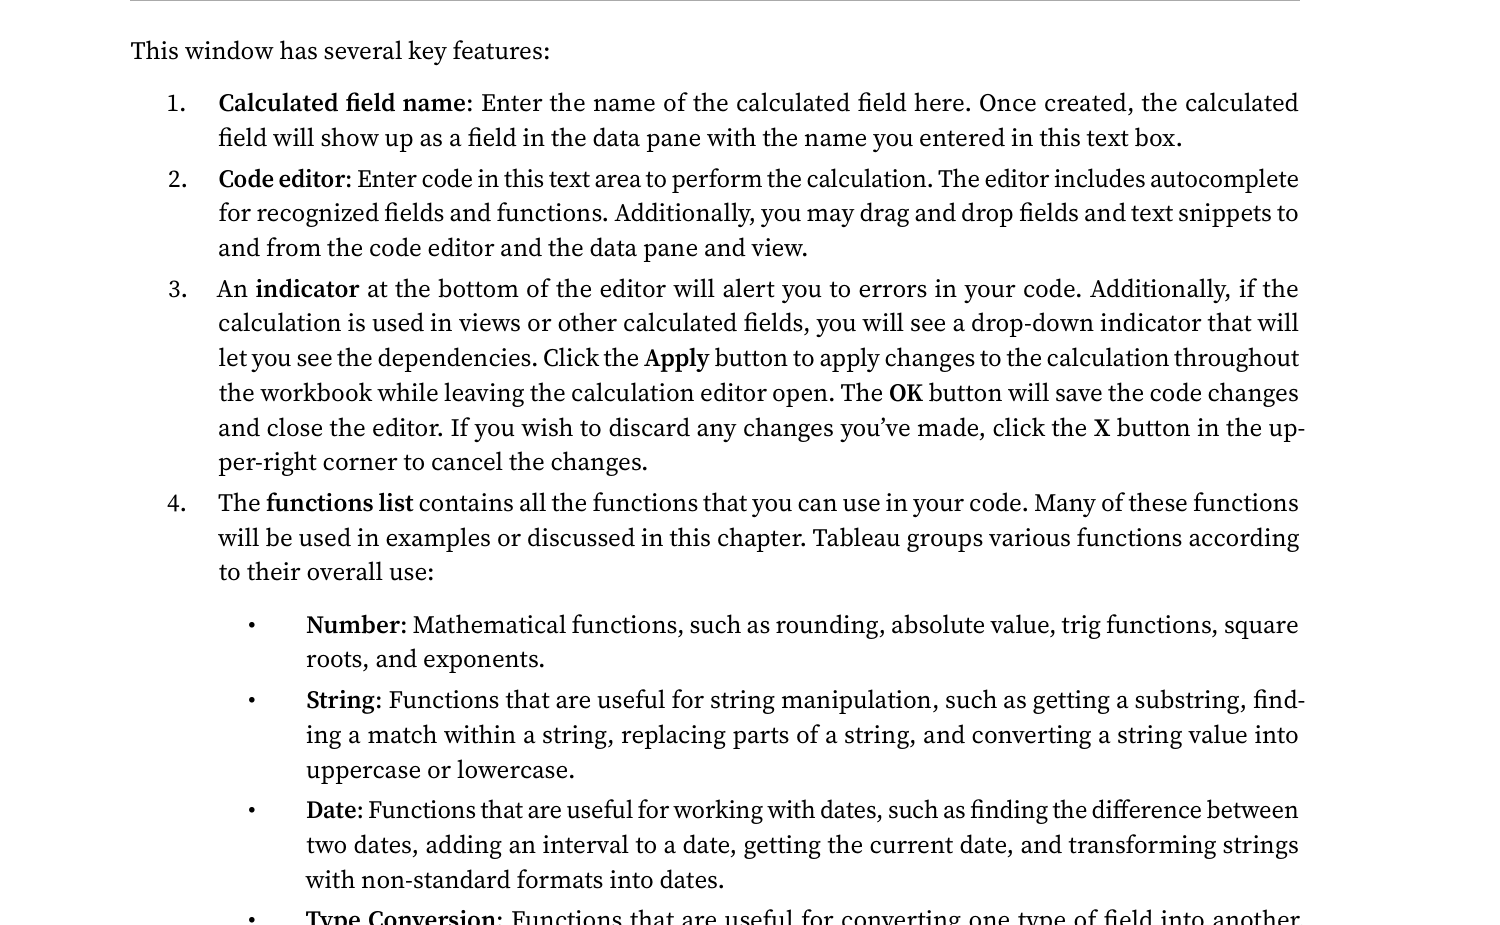
\includegraphics[width=0.9\linewidth]{images/calculated_field_functions.png}
\begin{figurecaptionmodern}
        \capfig{Cửa sổ Calculated Field --- các thành phần chính gồm: (1) ô nhập tên field, (2) vùng soạn code, (3) indicator lỗi, và (4) danh sách hàm phân loại theo Number, String, Date, Type Conversion...}
        \label{fig:calculated_field}
    \end{figurecaptionmodern}
\end{figure}

\noindent Trong phần này, chúng ta sẽ khám phá các hàm preprocessing được tổ chức theo \textbf{kiểu dữ liệu (data type)} --- vì mỗi kiểu có bộ hàm riêng phù hợp với đặc điểm của nó.

% ===================================================================
\subsection{Data Types trong Tableau}
% ===================================================================

\noindent Khi kết nối với nguồn dữ liệu, Tableau tự động phân tích và gán \textbf{kiểu dữ liệu (data type)} cho từng cột dựa trên nội dung của nó. Mỗi data type được nhận diện thông qua một \textbf{icon đặc trưng} hiển thị bên trái tên field trong Data Pane. Việc hiểu đúng data type cực kỳ quan trọng vì nó quyết định hàm nào có thể áp dụng, loại aggregation nào được phép, và biểu đồ nào Tableau sẽ gợi ý khi bạn drag field vào canvas.

\noindent Tableau hỗ trợ 6 data type cơ bản, được tóm tắt trong bảng sau:

\begin{center}
\renewcommand{\arraystretch}{1.4}
\begin{tabularx}{\linewidth}{c l X X}
\toprule
\textbf{Icon} & \textbf{Data Type} & \textbf{Mô tả} & \textbf{Ví dụ trong Superstore} \\
\midrule
\textbf{Abc} & \textbf{String} & Văn bản --- chuỗi ký tự bất kỳ & \texttt{Customer Name}, \texttt{Product Name}, \texttt{Region} \\
\textbf{\#} & \textbf{Number} & Số --- nguyên hoặc thập phân & \texttt{Sales}, \texttt{Profit}, \texttt{Quantity}, \texttt{Discount} \\
\faIcon{calendar} & \textbf{Date} & Ngày tháng --- chỉ có ngày, không có giờ & \texttt{Order Date}, \texttt{Ship Date} \\
\faIcon{calendar}\faIcon{clock} & \textbf{Date \& Time} & Ngày tháng kèm giờ phút giây & Dấu thời gian giao dịch hệ thống \\
\textbf{T|F} & \textbf{Boolean} & Nhị phân --- chỉ có True hoặc False & Kết quả so sánh, điều kiện lọc \\
\faIcon{globe} & \textbf{Geographic} & Địa lý --- Tableau tự nhận diện để vẽ bản đồ & \texttt{Country}, \texttt{State}, \texttt{City}, \texttt{Postal Code} \\
\bottomrule
\end{tabularx}
\end{center}

\begin{figure}[H]
\centering
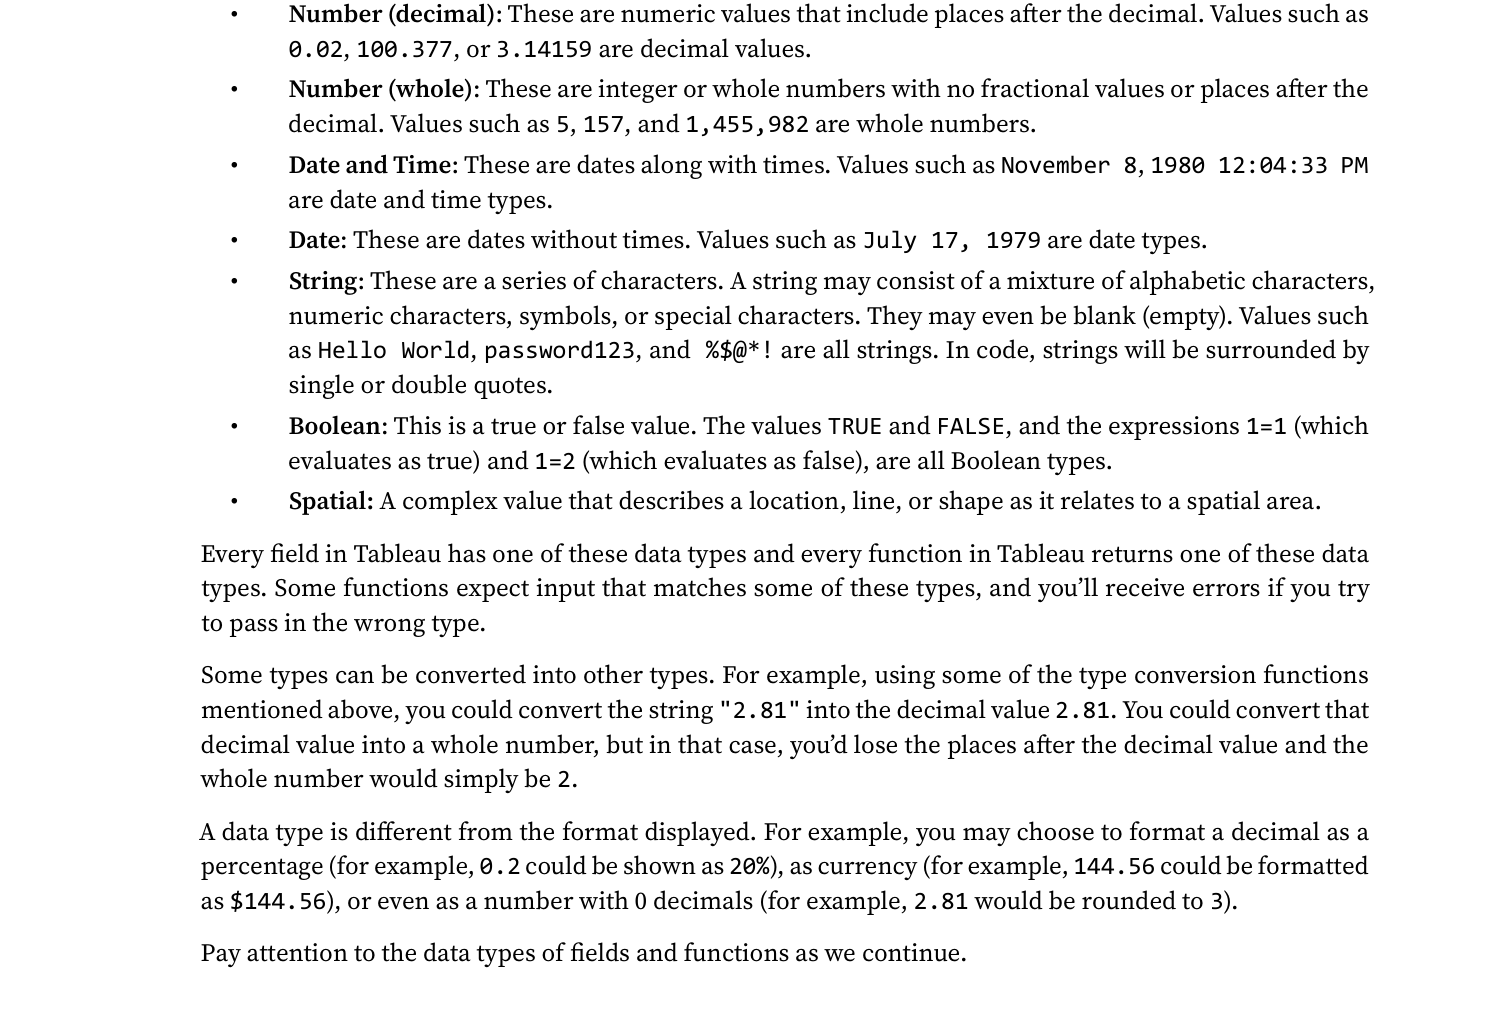
\includegraphics[width=0.9\linewidth]{images/data_types_list.png}
\begin{figurecaptionmodern}
        \capfig{Data Types trong Tableau --- giải thích chi tiết các kiểu dữ liệu: Number (decimal và whole), Date and Time, Date, String, Boolean, và Spatial.}
        \label{fig:data_types}
    \end{figurecaptionmodern}
\end{figure}

\begin{notebox}
\textbf{Tableau có thể nhận sai data type.} Tableau nhận diện data type dựa trên mẫu dữ liệu trong file, nhưng đôi khi mắc lỗi. Trường hợp phổ biến nhất là cột \texttt{Order Date} trong file CSV bị lưu với định dạng không chuẩn (\texttt{"15/1/2024"} thay vì \texttt{"2024-01-15"}) khiến Tableau nhận nhầm thành String --- mọi hàm ngày tháng sẽ thất bại.

\noindent \textbf{Cách kiểm tra nhanh:} Nhìn vào icon bên trái tên field trong Data Pane. Nếu thấy \textbf{Abc} cho một cột mà bạn biết là ngày tháng hoặc số, đó là dấu hiệu dữ liệu cần được chuyển đổi kiểu trước khi phân tích.
\end{notebox}

% ===================================================================
\subsection{Preprocessing Functions theo Data Type}
% ===================================================================

\noindent Tableau cung cấp hàng chục hàm preprocessing, được phân loại theo data type mà chúng xử lý. Trong thực tế, phần lớn các vấn đề tiền xử lý dữ liệu đều rơi vào 4 nhóm: \textbf{String}, \textbf{Number}, \textbf{Date}, và \textbf{Type Conversion}. Chúng ta sẽ đi sâu vào từng nhóm với bối cảnh thực tế và ví dụ cụ thể từ dataset Superstore.

% -------------------------------------------------------------------
\subsubsection{String Functions --- Xử lý văn bản}
% -------------------------------------------------------------------

\noindent Khi làm việc với dữ liệu thực tế, các trường văn bản thường là nguồn gốc của nhiều lỗi tinh vi nhất. Một cột \texttt{Customer Name} xuất từ hệ thống CRM có thể chứa khoảng trắng thừa ở đầu và cuối (do nhập liệu), viết hoa viết thường không nhất quán, hoặc thậm chí có ký tự đặc biệt không mong muốn. Những lỗi này không gây ra thông báo lỗi --- Tableau vẫn chạy bình thường --- nhưng kết quả phân tích sẽ sai: cùng một khách hàng nhưng bị đếm thành nhiều người khác nhau, filter không hoạt động đúng, hay group by ra kết quả thiếu.

\noindent Tableau cung cấp một bộ hàm String phong phú để giải quyết các vấn đề này. Dưới đây là các hàm thực dụng nhất mà một nhà phân tích dữ liệu cần nắm:

\begin{itemize}
    \item \textbf{\texttt{UPPER(string)} và \texttt{LOWER(string)}:} Chuyển đổi toàn bộ chuỗi sang chữ HOA hoặc chữ thường. Đây là thao tác chuẩn hóa đầu tiên khi cần so sánh hoặc nhóm dữ liệu văn bản --- \texttt{"Furniture"} và \texttt{"furniture"} là hai giá trị khác nhau trong Tableau, nhưng sau khi áp dụng \texttt{LOWER()} chúng sẽ hợp nhất thành một nhóm duy nhất.

    \item \textbf{\texttt{TRIM(string)}:} Xóa khoảng trắng ở \textbf{đầu và cuối} chuỗi --- không xóa khoảng trắng ở giữa. Đây là một trong những hàm quan trọng nhất vì khoảng trắng thừa hoàn toàn vô hình khi nhìn bằng mắt, nhưng khiến \texttt{"Hà Nội"} và \texttt{" Hà Nội"} trở thành hai chuỗi khác nhau và filter sẽ không khớp.

    \item \textbf{\texttt{LEFT(string, number)} và \texttt{RIGHT(string, number)}:} Trích xuất \texttt{n} ký tự từ bên trái hoặc bên phải của chuỗi. Ứng dụng phổ biến: trích xuất mã tỉnh/thành từ \texttt{"HN-001"} bằng \texttt{LEFT([City Code], 2)} để lấy \texttt{"HN"}.

    \item \textbf{\texttt{MID(string, start, length)}:} Trích xuất một đoạn con từ giữa chuỗi, bắt đầu từ vị trí \texttt{start} (1-indexed) với độ dài \texttt{length} ký tự. Ví dụ \texttt{"US-2024-00123"} --- ta có thể dùng \texttt{MID([Order ID], 4, 4)} để lấy năm \texttt{"2024"}.

    \item \textbf{\texttt{REPLACE(string, old, new)}:} Tìm và thay thế tất cả các lần xuất hiện của \texttt{old} bằng \texttt{new}. Ví dụ: \texttt{REPLACE([Phone], "-", "")} để xóa dấu gạch trong số điện thoại \texttt{"090-123-4567"} $\rightarrow$ \texttt{"0901234567"}.

    \item \textbf{\texttt{CONTAINS(string, substring)}:} Kiểm tra xem chuỗi có chứa chuỗi con không, trả về \texttt{True} hoặc \texttt{False}. Ví dụ: \texttt{CONTAINS([Product Name], "Chair")} trả về True cho tất cả sản phẩm có chữ ``Chair'' trong tên.

    \item \textbf{\texttt{LEN(string)}:} Đếm tổng số ký tự trong chuỗi. Thường dùng để kiểm tra dữ liệu: nếu mã sản phẩm phải có đúng 8 ký tự, \texttt{LEN([Product ID]) != 8} sẽ phát hiện các mã bị lỗi.

    \item \textbf{\texttt{SPLIT(string, delimiter, token\_number)}:} Tách chuỗi thành các phần dựa trên ký tự phân cách và lấy phần thứ \texttt{token\_number}. Ví dụ \texttt{SPLIT("Furniture/Bookcases", "/", 2)} trả về \texttt{"Bookcases"}.

    \item \textbf{Toán tử nối chuỗi \texttt{+}:} Dấu cộng \texttt{+} dùng để \textbf{ghép nối (concatenate)} các chuỗi. Ví dụ: \texttt{[First Name] + " " + [Last Name]} tạo ra \texttt{"Claire Gute"}. Lưu ý: \textbf{phải thêm khoảng trắng thủ công} vào công thức (\texttt{+ " " +}).

    \item \textbf{\texttt{STARTSWITH(string, substring)}:} Kiểm tra xem chuỗi có \textbf{bắt đầu} bằng chuỗi con không, trả về \texttt{True/False}. \texttt{STARTSWITH([Order ID], "US")} trả về True cho tất cả đơn hàng có mã bắt đầu bằng ``US''.

    \item \textbf{\texttt{ENDSWITH(string, substring)}:} Kiểm tra xem chuỗi có \textbf{kết thúc} bằng chuỗi con không. \texttt{ENDSWITH([File Name], ".csv")} trả về True cho các file CSV.

    \item \textbf{\texttt{FIND(string, substring, [start])}:} Tìm vị trí của chuỗi con trong chuỗi --- trả về số thứ tự ký tự (1-indexed), hoặc \textbf{0 nếu không tìm thấy}. Ví dụ: \texttt{FIND("CA-2024-01", "-")} = 3.

    \item \textbf{\texttt{LTRIM(string)} và \texttt{RTRIM(string)}:} Xóa khoảng trắng \textbf{chỉ bên trái} (\texttt{LTRIM}) hoặc \textbf{chỉ bên phải} (\texttt{RTRIM}) --- chi tiết hơn \texttt{TRIM()} vốn xóa cả 2 phía.
\end{itemize}

\noindent \textbf{Ví dụ tổng hợp --- Chuẩn hóa tên khách hàng:}

\noindent Giả sử trường \texttt{Customer Name} trong Superstore có giá trị lộn xộn như \texttt{"~~CLAIRE GUTE~~"} (thừa khoảng trắng, toàn chữ hoa). Chúng ta tạo một Calculated Field mới tên \texttt{[Customer Name Cleaned]}:

\begin{aivncodebox}[]
\begin{python}
// Xóa khoảng trắng dư + chuyển về chữ thường để chuẩn hóa so sánh
LOWER(TRIM([Customer Name]))

// Kết quả: "claire gute"
\end{python}
\end{aivncodebox}

\noindent Hoặc nếu muốn kiểm tra nhanh tên nào còn khoảng trắng thừa (để lọc ra dữ liệu lỗi):

\begin{aivncodebox}[]
\begin{python}
// True = có khoảng trắng thừa ở đầu hoặc cuối
LEN([Customer Name]) != LEN(TRIM([Customer Name]))

// Kết quả: True / False
\end{python}
\end{aivncodebox}

\begin{figure}[H]
\centering
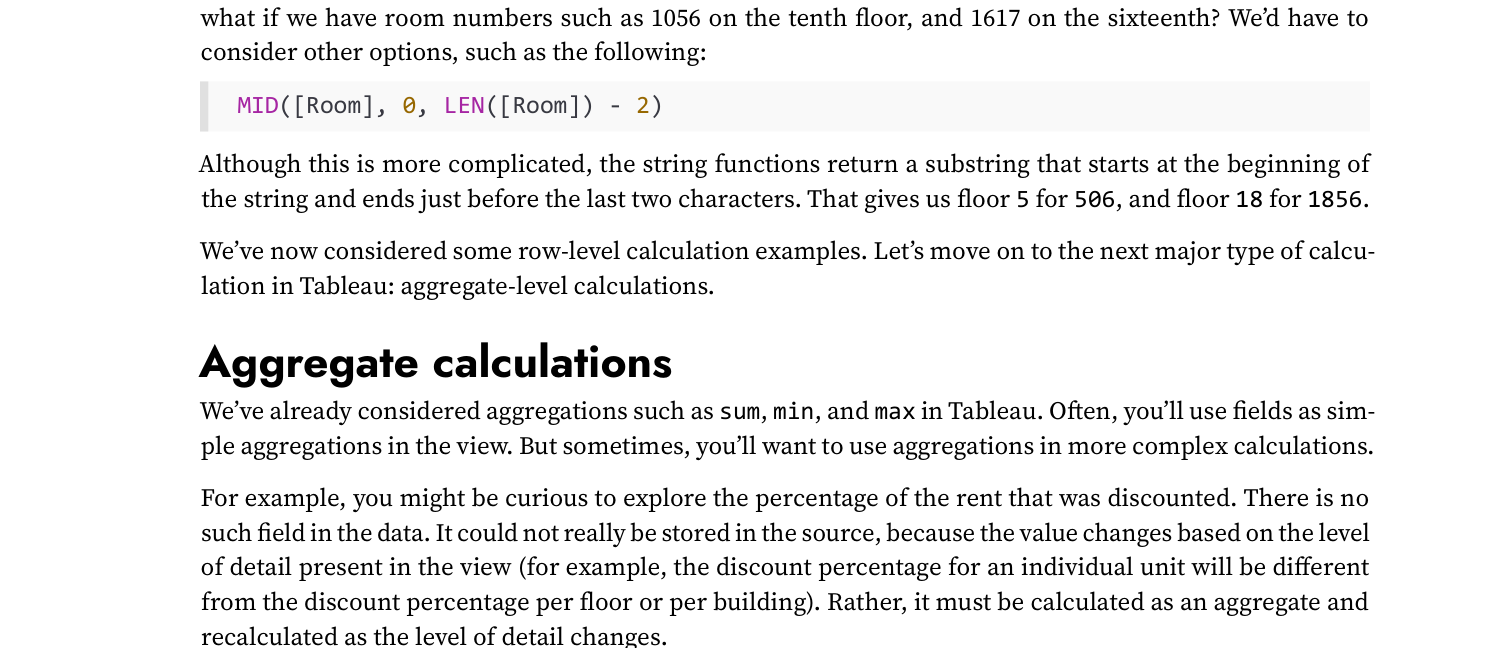
\includegraphics[width=0.9\linewidth]{images/string_functions_example.png}
\begin{figurecaptionmodern}
        \capfig{Ví dụ String Functions --- sử dụng \texttt{MID} và \texttt{LEN} để trích xuất thông tin từ chuỗi. Mã màu cú pháp giúp phân biệt tên hàm (xanh), tên field (cam), và hằng số (tím).}
        \label{fig:string_functions}
    \end{figurecaptionmodern}
\end{figure}

\begin{guidelinebox}{Tableau không có hàm PROPER()}
Python có \texttt{str.title()} và Excel có \texttt{PROPER()} để viết hoa chữ cái đầu mỗi từ, nhưng Tableau không có hàm tương đương sẵn có.

\noindent Workaround đơn giản cho tên một từ: \texttt{UPPER(LEFT([Name], 1)) + LOWER(MID([Name], 2, LEN([Name])))}

\noindent Tuy nhiên với tên nhiều từ (như tên người), workaround này chỉ viết hoa được từ đầu tiên. Đối với trường hợp này, tốt hơn nên xử lý bằng Python trước khi import vào Tableau.
\end{guidelinebox}

% -------------------------------------------------------------------
\subsubsection{Number Functions --- Xử lý số}
% -------------------------------------------------------------------

\noindent Dữ liệu số trong Tableau ít gặp lỗi về kiểu hơn String, nhưng vẫn cần xử lý trong nhiều tình huống: làm tròn để hiển thị gọn gàng, lấy trị tuyệt đối khi chỉ quan tâm độ lớn, hay xử lý giá trị NULL khiến mọi phép tính đều trả về NULL thay vì giá trị thực.

\noindent Trong dataset Superstore, trường \texttt{Profit} là ví dụ điển hình --- nó có thể mang giá trị âm khi đơn hàng bị lỗ, và trường \texttt{Discount} thường là số thập phân (0.1, 0.2, ...) cần làm tròn khi hiển thị. Dưới đây là các hàm Number thực dụng nhất:

\begin{itemize}
    \item \textbf{\texttt{ROUND(number, decimal\_places)}:} Làm tròn đến số chữ số thập phân chỉ định. \texttt{ROUND([Sales], 2)} làm tròn doanh thu đến 2 chữ số thập phân. Khi \texttt{decimal\_places = 0}, hàm làm tròn về số nguyên gần nhất. Khi \texttt{decimal\_places} là số âm, hàm làm tròn về hàng chục, hàng trăm... ví dụ \texttt{ROUND(1234, -2)} = 1200.

    \item \textbf{\texttt{CEILING(number)} và \texttt{FLOOR(number)}:} Hai hàm làm tròn ``lệch'' --- \texttt{CEILING()} luôn làm tròn \textbf{lên} đến số nguyên tiếp theo (ví dụ \texttt{CEILING(3.2)} = 4), còn \texttt{FLOOR()} luôn làm tròn \textbf{xuống} (ví dụ \texttt{FLOOR(3.8)} = 3). Hữu ích trong các bài toán phân nhóm hay làm tròn giá vé, chi phí vận chuyển.

    \item \textbf{\texttt{ABS(number)}:} Trả về giá trị tuyệt đối --- bỏ dấu âm. \texttt{ABS([Profit])} cho biết độ lớn của lãi/lỗ bất kể chiều hướng. Thường dùng: \texttt{ABS([Actual] - [Target])}.

    \item \textbf{\texttt{ZN(expression)}:} Viết tắt của \textbf{``Zero if Null''} --- nếu biểu thức trả về NULL thì thay bằng 0, ngược lại giữ nguyên giá trị. Đây là một trong những hàm quan trọng nhất khi làm việc với dữ liệu có missing values, vì trong Tableau bất kỳ phép tính nào có NULL đều trả về NULL: \texttt{NULL + 100 = NULL}, \texttt{NULL * 5 = NULL}.

    \item \textbf{\texttt{POWER(number, exponent)}:} Tính lũy thừa. \texttt{POWER([Sales], 2)} = Sales bình phương. Cần thiết khi tính các chỉ số thống kê hoặc chuẩn hóa dữ liệu.

    \item \textbf{\texttt{SIGN(number)}:} Trả về \textbf{--1} nếu số âm, \textbf{0} nếu bằng 0, \textbf{1} nếu dương. Kết hợp với CASE: \texttt{CASE SIGN([Profit]) WHEN 1 THEN "Lãi" WHEN -1 THEN "Lỗ" ELSE "Hòa vốn" END}.

    \item \textbf{\texttt{DIV(integer1, integer2)}:} Chia nguyên --- trả về phần nguyên của phép chia. \texttt{DIV(7, 2)} = 3 (không phải 3.5). Hữu ích khi tính số lô hàng nguyên: \texttt{DIV([Quantity], [Batch Size])}.
\end{itemize}

\noindent \textbf{Ví dụ tổng hợp --- Phân loại đơn hàng theo lợi nhuận:}

\begin{aivncodebox}[]
\begin{python}
// Phân loại đơn hàng: Lãi, Huề vốn, hoặc Lỗ
IF [Profit] > 0 THEN "Profitable"
ELSEIF [Profit] = 0 THEN "Break-even"
ELSE "Loss"
END

// Kết quả: "Profitable" / "Break-even" / "Loss" cho từng dòng
\end{python}
\end{aivncodebox}

\noindent Và tính \textbf{tỷ suất lợi nhuận (profit margin)} một cách an toàn, tránh lỗi chia cho 0:

\begin{aivncodebox}[]
\begin{python}
// ZN đảm bảo khi Sales = NULL thì kết quả = 0 thay vì NULL
ZN([Profit]) / ZN([Sales])

// Hoặc viết cẩn thận hơn để tránh lỗi chia cho 0:
IF ZN([Sales]) = 0 THEN 0
ELSE [Profit] / [Sales]
END
\end{python}
\end{aivncodebox}

\begin{notebox}
\textbf{NULL trong Tableau $\neq$ 0.} Đây là một trong những điểm gây nhầm lẫn phổ biến nhất. Trong Tableau, NULL không phải là 0 --- nó là ``không có dữ liệu''. Mọi phép tính số học với NULL đều trả về NULL, không phải một số.

\noindent Ví dụ thực tế: Nếu một khách hàng chưa có đơn hàng nào trong tháng, trường \texttt{Sales} của họ là NULL (không phải 0). \texttt{SUM(NULL, 50, 30)} = 80 --- hàm SUM bỏ qua NULL. Nhưng \texttt{NULL / 100} = NULL --- phép chia thất bại. Luôn dùng \texttt{ZN()} trước khi thực hiện phép chia để đảm bảo an toàn.
\end{notebox}

% -------------------------------------------------------------------
\subsubsection{Date Functions --- Xử lý ngày tháng}
% -------------------------------------------------------------------

\noindent Phân tích theo thời gian là một trong những yêu cầu phổ biến nhất trong Business Intelligence. Với dataset Superstore có hai trường date là \texttt{Order Date} và \texttt{Ship Date}, chúng ta cần khả năng: tách năm/quý/tháng để nhóm dữ liệu, tính khoảng cách giữa ngày đặt hàng và ngày giao hàng, hay lọc ra các đơn hàng trong 30 ngày gần nhất so với ngày hôm nay.

\noindent Trước khi bắt đầu, cần hiểu khái niệm quan trọng nhất trong Date Functions --- tham số \textbf{\texttt{date\_part}}. Đây là một chuỗi chỉ định \textbf{đơn vị thời gian} mà hàm sẽ làm việc với:

\begin{center}
\renewcommand{\arraystretch}{1.4}
\begin{tabularx}{\linewidth}{l l X}
\toprule
\textbf{Giá trị \texttt{date\_part}} & \textbf{Ý nghĩa} & \textbf{Kết quả (ví dụ với 15/03/2024)} \\
\midrule
\texttt{'year'} & Năm & 2024 \\
\texttt{'quarter'} & Quý trong năm & 1 (Q1: tháng 1--3) \\
\texttt{'month'} & Tháng trong năm & 3 \\
\texttt{'day'} & Ngày trong tháng & 15 \\
\texttt{'weekday'} & Thứ trong tuần & 6 (6 = Thứ Sáu, ISO) \\
\texttt{'hour'} & Giờ (chỉ dùng với Date \& Time) & 0--23 \\
\bottomrule
\end{tabularx}
\end{center}

\noindent Các hàm Date thực dụng nhất trong phân tích dữ liệu bán hàng:

\begin{itemize}
    \item \textbf{\texttt{YEAR(date)}, \texttt{MONTH(date)}, \texttt{DAY(date)}:} Ba hàm đơn giản nhất để trích xuất năm, tháng, ngày từ một trường Date. \texttt{YEAR([Order Date])} trả về số nguyên như 2021, 2022... Đây là cách nhanh nhất để tạo các trường phụ trợ phục vụ nhóm dữ liệu theo thời gian.

    \item \textbf{\texttt{DATEPART(date\_part, date)}:} Tổng quát hơn \texttt{YEAR/MONTH/DAY} --- có thể lấy bất kỳ đơn vị thời gian nào. \texttt{DATEPART('quarter', [Order Date])} trả về 1, 2, 3, hoặc 4. Kết quả là \textbf{số nguyên}, phù hợp cho tính toán.

    \item \textbf{\texttt{DATENAME(date\_part, date)}:} Tương tự \texttt{DATEPART} nhưng trả về \textbf{tên dạng chuỗi}. \texttt{DATENAME('month', [Order Date])} trả về \texttt{"January"}, \texttt{"February"}... Hữu ích khi muốn hiển thị nhãn thân thiện trên biểu đồ.

    \item \textbf{\texttt{DATEDIFF(date\_part, start\_date, end\_date)}:} Tính \textbf{khoảng cách} giữa hai ngày. \texttt{DATEDIFF('day', [Order Date], [Ship Date])} cho biết mất bao nhiêu ngày để giao hàng.

    \item \textbf{\texttt{DATEADD(date\_part, interval, date)}:} Cộng (hoặc trừ nếu \texttt{interval} âm) một khoảng thời gian vào một ngày. \texttt{DATEADD('month', 3, [Order Date])} trả về ngày 3 tháng sau ngày đặt hàng.

    \item \textbf{\texttt{TODAY()}:} Trả về ngày hôm nay (không có giờ). Thường kết hợp với \texttt{DATEDIFF} để tạo filter động.

    \item \textbf{\texttt{DATETRUNC(date\_part, date)}:} ``Cắt'' ngày về \textbf{đầu kỳ} tương ứng. \texttt{DATETRUNC('month', \#2024-03-15\#)} = \textbf{1/3/2024}; \texttt{DATETRUNC('quarter', \#2024-03-15\#)} = \textbf{1/1/2024}. Cực kỳ hữu ích khi cần so sánh các kỳ với nhau.

    \item \textbf{\texttt{NOW()}:} Trả về \textbf{ngày và giờ hiện tại} (Date \& Time) --- khác với \texttt{TODAY()} chỉ trả về ngày. Lưu ý: \texttt{NOW()} tính theo múi giờ của máy chủ Tableau, không phải browser người dùng.

    \item \textbf{\texttt{QUARTER(date)} và \texttt{WEEK(date)}:} Shorthand nhanh --- \texttt{QUARTER([Order Date])} trả về 1--4; \texttt{WEEK([Order Date])} trả về số tuần trong năm (1--52/53).

    \item \textbf{\texttt{MAKEDATE(year, month, day)}:} Tạo một giá trị Date từ 3 số nguyên riêng lẻ. \texttt{MAKEDATE(2024, 3, 15)} tạo ngày 15/3/2024. Hữu ích khi dữ liệu lưu riêng năm, tháng, ngày trong 3 cột Number.

    \item \textbf{\texttt{DATEPARSE(format, string)}:} Chuyển đổi một \textbf{chuỗi} có định dạng đặc biệt thành kiểu Date. Ví dụ:
\end{itemize}

\begin{aivncodebox}[]
\begin{python}
DATEPARSE("MMMM,d,yy", "September,4,12")
// Kết quả: 9/4/2012 (ngày tháng năm theo ISO)
\end{python}
\end{aivncodebox}

\noindent Các định dạng phổ biến: \texttt{yyyy} = năm 4 chữ số, \texttt{MM} = tháng 2 chữ số, \texttt{dd} = ngày 2 chữ số, \texttt{MMMM} = tên tháng đầy đủ, \texttt{MMM} = tên tháng viết tắt. Chuỗi format phải \textbf{khớp chính xác} với cấu trúc của chuỗi ngày.

\noindent \textbf{Ví dụ tổng hợp --- Phân tích thời gian giao hàng:}

\begin{aivncodebox}[]
\begin{python}
// Tính số ngày giao hàng (từ Order Date đến Ship Date)
DATEDIFF('day', [Order Date], [Ship Date])
// Kết quả: 2, 3, 5... (số nguyên)

// Phân loại tốc độ giao hàng
IF DATEDIFF('day', [Order Date], [Ship Date]) <= 2
THEN "Fast"
ELSEIF DATEDIFF('day', [Order Date], [Ship Date]) <= 5
THEN "Normal (3-5 days)"
ELSE "Slow (>5 days)"
END

// Lọc đơn hàng trong 365 ngày gần nhất
DATEDIFF('day', [Order Date], TODAY()) <= 365
// Kết quả: True / False — dùng làm filter condition
\end{python}
\end{aivncodebox}

\begin{guidelinebox}{DATEPART vs DATENAME: khi nào dùng cái nào?}
\begin{itemize}[nosep]
    \item Dùng \textbf{\texttt{DATEPART('month', ...)}} $\rightarrow$ kết quả là số \texttt{1, 2, ..., 12} $\rightarrow$ khi cần \textbf{tính toán} (so sánh, cộng trừ)
    \item Dùng \textbf{\texttt{DATENAME('month', ...)}} $\rightarrow$ kết quả là \texttt{"January", "February", ...} $\rightarrow$ khi cần \textbf{hiển thị nhãn} trên trục X
\end{itemize}
\noindent Lưu ý: kết quả của \texttt{DATENAME} sẽ sắp xếp theo bảng chữ cái (April, August, December...) thay vì theo thứ tự tháng. Để sắp xếp đúng, hãy dùng thêm \texttt{DATEPART} làm trường sắp xếp phụ trợ (Sort Field).
\end{guidelinebox}

% -------------------------------------------------------------------
\subsubsection{Ad-hoc Calculations và xử lý giá trị NULL}
% -------------------------------------------------------------------

\noindent Ngoài việc tạo Calculated Field đầy đủ qua menu \textbf{Analysis $\rightarrow$ Create Calculated Field...}, Tableau còn hỗ trợ một cách tạo công thức nhanh hơn gọi là \textbf{Ad-hoc Calculation}. Phương pháp này cho phép nhập công thức \textbf{trực tiếp trên Columns shelf, Rows shelf, hoặc thẻ Marks} mà không cần đặt tên hay lưu lại.

\noindent \textbf{Cách tạo Ad-hoc Calculation:}
\begin{enumerate}[nosep]
    \item Kéo field \texttt{Profit} vào Columns shelf. Tableau hiển thị \texttt{SUM([Profit])}.
    \item Nhấp đúp vào pill \texttt{SUM([Profit])} trên Columns shelf --- một ô nhập công thức nhỏ xuất hiện.
    \item Sửa thành \texttt{SUM([Profit])/SUM([Sales])} và nhấn \textbf{Enter}. Tableau tính và hiển thị kết quả ngay lập tức.
    \item Nếu muốn lưu lại: kéo pill từ shelf vào \textbf{Data Pane}, Tableau sẽ yêu cầu đặt tên cho Calculated Field.
\end{enumerate}

\noindent Tableau có hệ thống \textbf{mã màu cú pháp} trong Formula Editor:

\begin{center}
\renewcommand{\arraystretch}{1.4}
\begin{tabularx}{\linewidth}{l X}
\toprule
\textbf{Màu/kiểu chữ} & \textbf{Ý nghĩa} \\
\midrule
\textbf{Chữ đỏ} (gạch chân) & Lỗi cú pháp --- di chuột lên để xem gợi ý sửa \\
\texttt{// chữ màu xám} & Comment --- không ảnh hưởng tính toán \\
\textbf{[chữ màu cam]} & Tên field --- cần bao bằng dấu \texttt{[]} \\
\textbf{chữ màu xanh} & Tên hàm (function) \\
\textbf{[chữ màu tím]} & Parameters \\
\textbf{chữ in đậm} & Phép tính được aggregate \\
chữ không in đậm & Phép tính ở mức row-level \\
\bottomrule
\end{tabularx}
\end{center}

\noindent \textbf{Xử lý giá trị NULL với \texttt{ZN()}:}

\noindent Khi kết hợp hoặc trộn lẫn nhiều nguồn dữ liệu, một số ô có thể không có giá trị (NULL). Trong Tableau, \texttt{NULL + bất kì số nào = NULL} --- nghĩa là một giá trị NULL duy nhất sẽ làm cho toàn bộ kết quả là NULL.

\noindent \textbf{Hàm \texttt{ZN(expression)}} (Zero-if-Null) giải quyết vấn đề này:

\begin{aivncodebox}[]
\begin{python}
// Không an toàn: nếu Discount là NULL, kết quả sẽ là NULL
[Sales] * [Discount]

// An toàn: ZN thay NULL bằng 0 trước
ZN([Sales]) * ZN([Discount])
\end{python}
\end{aivncodebox}

\noindent Lưu ý: \texttt{ZN} chỉ dùng đối với số (Number) --- thay NULL số bằng 0 thường hợp lý (không có Discount có nghĩa Discount = 0\%), nhưng cần cân nhắc kỹ trong ngữ cảnh cụ thể.

% -------------------------------------------------------------------
\subsubsection{Type Conversion Functions --- Chuyển đổi kiểu dữ liệu}
% -------------------------------------------------------------------

\noindent Một trong những vấn đề phổ biến nhất khi import dữ liệu vào Tableau là \textbf{kiểu dữ liệu bị nhận sai}. Nguyên nhân thường gặp: file CSV có cột số nhưng chứa ký tự không phải số (dấu phẩy \texttt{"1,234.56"}, đơn vị tiền tệ \texttt{"\$500"}), cột ngày tháng có định dạng không chuẩn, hoặc Tableau đọc toàn bộ cột là String vì có một vài ô chứa chữ.

\noindent Khi dữ liệu bị nhận sai kiểu, hậu quả rất rõ ràng: không thể tính \texttt{SUM([Revenue])} nếu Revenue là String, không thể dùng \texttt{YEAR([Order Date])} nếu Order Date là String. Type Conversion Functions cho phép chúng ta ép kiểu (cast) dữ liệu sang đúng loại:

\begin{itemize}
    \item \textbf{\texttt{INT(expression)}:} Chuyển đổi sang số nguyên, cắt bỏ phần thập phân (không làm tròn --- \texttt{INT(3.9)} = 3, không phải 4).

    \item \textbf{\texttt{FLOAT(expression)}:} Chuyển đổi sang số thực (có phần thập phân). Phổ biến hơn \texttt{INT} vì giữ được độ chính xác. \texttt{FLOAT("1234.56")} trả về số \texttt{1234.56}.

    \item \textbf{\texttt{STR(expression)}:} Chuyển đổi \textbf{sang String}. Hữu ích khi cần ghép Number vào chuỗi: \texttt{"Order \#" + STR([Order ID])} tạo ra \texttt{"Order \#12345"}.

    \item \textbf{\texttt{DATE(expression)}:} Chuyển đổi String hoặc Number sang kiểu Date. \texttt{DATE("2024-01-15")} trả về ngày 15/1/2024 với đầy đủ khả năng sử dụng các Date Functions.

    \item \textbf{\texttt{DATETIME(expression)}:} Tương tự \texttt{DATE()} nhưng tạo ra giá trị Date \& Time, bao gồm cả giờ phút giây.
\end{itemize}

\noindent \textbf{Ví dụ tổng hợp --- Sửa cột dữ liệu bị nhận sai kiểu:}

\begin{aivncodebox}[]
\begin{python}
// Trường hợp 1: Cột "Revenue_str" = "1234.56" (String)
// -> Chuyển thành Number để có thể SUM, AVG
FLOAT([Revenue_str])
// Kết quả: 1234.56

// Trường hợp 2: Cột "Order_Date_str" = "2024-01-15" (String)
// -> Chuyển thành Date để dùng YEAR(), DATEDIFF()...
DATE([Order_Date_str])
// Kết quả: 15/01/2024 (Date)

// Trường hợp 3: Tạo label kết hợp số và chữ
"Đơn hàng #" + STR([Order ID]) + " — " + STR([Customer Name])
// Kết quả: "Đơn hàng #12345 — Claire Gute"
\end{python}
\end{aivncodebox}

\begin{notebox}
\textbf{Nhận biết lỗi kiểu dữ liệu ngay từ đầu ---} Có 3 dấu hiệu rõ ràng:
\begin{enumerate}[nosep]
    \item Field có icon \textbf{Abc} trong Data Pane nhưng bạn biết nó là số hoặc ngày
    \item Tableau báo lỗi \textbf{``Cannot mix aggregate and non-aggregate arguments''} khi bạn cố tính SUM
    \item Tableau không gợi ý \textbf{Line Chart} khi bạn drag một Date field vào Columns
\end{enumerate}
\noindent Bước xử lý chuẩn: tạo Calculated Field mới dùng \texttt{FLOAT()}, \texttt{DATE()}, hay \texttt{INT()} để chuyển đổi, đặt tên rõ ràng (ví dụ \texttt{[Sales (Numeric)]}), rồi sử dụng field mới đó thay cho field gốc.
\end{notebox}

% -------------------------------------------------------------------
\subsubsection{Logical Functions --- Phân loại và điều kiện hóa dữ liệu}
% -------------------------------------------------------------------

\noindent Nếu String Functions giúp làm sạch dữ liệu và Date Functions giúp phân tích thời gian, thì \textbf{Logical Functions} là trái tim của mọi phân tích dữ liệu có chiều sâu --- chúng cho phép Tableau đưa ra \textbf{quyết định} dựa trên điều kiện, phân loại dữ liệu thành nhóm, và xử lý các trường hợp đặc biệt.

\paragraph{IF / ELSEIF / ELSE / END --- Điều kiện nhiều nhánh}

\noindent Cú pháp IF là cách phổ biến nhất để phân loại dữ liệu trong Tableau:

\begin{aivncodebox}[]
\begin{python}
IF <test1> THEN <value1>
ELSEIF <test2> THEN <value2>
...
ELSE <default_value>
END
\end{python}
\end{aivncodebox}

\begin{itemize}[nosep]
    \item Tableau kiểm tra \textbf{lần lượt} từng điều kiện, trả về giá trị tương ứng với điều kiện đầu tiên là \texttt{True}
    \item \texttt{ELSEIF} và \texttt{ELSE} là tùy chọn --- có thể viết \texttt{IF...THEN...END} đơn giản
    \item Phần \texttt{ELSE} là giá trị mặc định khi không có điều kiện nào khớp --- nếu bỏ qua, kết quả là \texttt{NULL}
\end{itemize}

\noindent \textbf{Ví dụ thực tế --- Phân loại lợi nhuận:}

\begin{aivncodebox}[]
\begin{python}
// Tạo Calculated Field [Profit Status]
IF [Profit] > 0 THEN "Profitable"
ELSEIF [Profit] = 0 THEN "Break-even"
ELSE "Loss"
END
\end{python}
\end{aivncodebox}

\noindent \textbf{Ví dụ nâng cao --- Phân loại theo nhiều trường:}

\begin{aivncodebox}[]
\begin{python}
// Phân loại khách hàng VIP dựa trên cả Sales và Profit
IF SUM([Sales]) > 10000 AND SUM([Profit]) > 1000
THEN "VIP"
ELSEIF SUM([Sales]) > 5000
THEN "Regular"
ELSE "New"
END

// Lưu ý: Khi dùng IF kết hợp aggregate (SUM),
// cả công thức phải ở cấp aggregate
\end{python}
\end{aivncodebox}

\begin{conceptbox}{IIF (Inline IF)}
\texttt{IIF(<test>, <then>, <else>)} là phiên bản rút gọn của IF cho trường hợp chỉ có 2 nhánh. \texttt{IIF([Profit] > 0, "Lãi", "Lỗ")} tương đương với \texttt{IF [Profit] > 0 THEN "Lãi" ELSE "Lỗ" END}. Dùng khi công thức đơn giản --- nhưng khi cần nhiều điều kiện, IF/ELSEIF dễ đọc hơn nhiều IIF lồng nhau.
\end{conceptbox}

\paragraph{CASE / WHEN / THEN --- Phân loại theo giá trị cụ thể}

\noindent CASE là lựa chọn tốt hơn IF khi bạn cần so sánh \textbf{một field với nhiều giá trị cụ thể}:

\begin{aivncodebox}[]
\begin{python}
CASE <expression>
WHEN <value1> THEN <result1>
WHEN <value2> THEN <result2>
...
[ELSE <default>]
END
\end{python}
\end{aivncodebox}

\noindent \textbf{Ví dụ thực tế --- Dịch tên vùng sang tiếng Việt:}

\begin{aivncodebox}[]
\begin{python}
CASE [Region]
WHEN "East" THEN "Miền Đông"
WHEN "West" THEN "Miền Tây"
WHEN "North" THEN "Miền Bắc"
WHEN "South" THEN "Miền Nam"
ELSE "Không xác định"
END
\end{python}
\end{aivncodebox}

\begin{guidelinebox}{IF vs CASE: khi nào dùng cái nào?}
\renewcommand{\arraystretch}{1.3}
\begin{tabularx}{\linewidth}{X X}
\toprule
\textbf{CASE} & \textbf{IF} \\
\midrule
So sánh \textbf{một field} với nhiều \textbf{giá trị rời rạc} & Kiểm tra \textbf{nhiều điều kiện phức tạp} khác nhau \\
\texttt{[Region] = "East"}, \texttt{[Region] = "West"}... & \texttt{[Sales] > 10000 AND [Profit] > 0}... \\
Cú pháp gọn hơn, dễ đọc hơn & Linh hoạt hơn --- dùng được \texttt{>}, \texttt{<}, \texttt{AND}, \texttt{OR} \\
\bottomrule
\end{tabularx}
\end{guidelinebox}

\paragraph{Toán tử logic: AND, OR, NOT}

\noindent Các toán tử này kết hợp nhiều điều kiện vào một biểu thức:

\begin{itemize}
    \item \textbf{\texttt{AND}:} Cả hai điều kiện đều phải \texttt{True}. \texttt{[Sales] > 1000 AND [Profit] > 0} --- chỉ đơn hàng lãi VÀ có doanh thu cao. AND dùng \textbf{short-circuit evaluation}.

    \item \textbf{\texttt{OR}:} Chỉ cần một trong hai điều kiện là \texttt{True}. \texttt{[Region] = "East" OR [Region] = "West"}.

    \item \textbf{\texttt{NOT}:} Đảo ngược kết quả boolean. \texttt{NOT ISNULL([Customer ID])} --- chỉ giữ lại các dòng có Customer ID.
\end{itemize}

\begin{aivncodebox}[]
\begin{python}
// Ví dụ kết hợp: đơn hàng cần chú ý
// (Lỗ lớn HOẶC chiết khấu cao) VÀ không phải khách VIP
(SUM([Profit]) < -500 OR SUM([Discount]) > 0.3)
AND NOT ([Customer Segment] = "VIP")
\end{python}
\end{aivncodebox}

\paragraph{Xử lý NULL: ISNULL, IFNULL và ZN}

\noindent Ba hàm xử lý NULL trong Tableau, mỗi hàm phục vụ mục đích khác nhau:

\begin{center}
\renewcommand{\arraystretch}{1.4}
\begin{tabularx}{\linewidth}{l l l X}
\toprule
\textbf{Hàm} & \textbf{Cú pháp} & \textbf{Trả về} & \textbf{Dùng khi} \\
\midrule
\textbf{\texttt{ISNULL}} & \texttt{ISNULL(expr)} & \texttt{True/False} & Cần \textbf{kiểm tra} xem field có NULL không \\
\textbf{\texttt{IFNULL}} & \texttt{IFNULL(e1, e2)} & Giá trị e1 hoặc e2 & Cần \textbf{thay thế NULL bằng giá trị bất kỳ} \\
\textbf{\texttt{ZN}} & \texttt{ZN(expr)} & Giá trị hoặc \textbf{0} & Cần \textbf{thay NULL bằng 0} cho phép tính số \\
\bottomrule
\end{tabularx}
\end{center}

\begin{aivncodebox}[]
\begin{python}
// ISNULL — Phát hiện dữ liệu thiếu
ISNULL([Customer ID])
// Kết quả: True cho các dòng chưa có Customer ID

// IFNULL — Thay NULL bằng giá trị mặc định có nghĩa
IFNULL([Assigned Region], "Chưa phân vùng")
// Kết quả: Chuỗi thực hoặc "Chưa phân vùng"

// ZN — Đảm bảo an toàn cho phép tính số
ZN([Discount]) * ZN([Sales])
// Kết quả: Nếu NULL -> kết quả là 0, không phải NULL
\end{python}
\end{aivncodebox}

\begin{notebox}
\textbf{IFNULL vs ZN vs ISNULL:}
\begin{itemize}[nosep]
    \item \texttt{ISNULL} chỉ \textbf{phát hiện} (trả Boolean), không thay thế
    \item \texttt{IFNULL} thay NULL bằng \textbf{bất kỳ giá trị nào} (String, Number, Date...)
    \item \texttt{ZN} chỉ thay bằng \textbf{0} --- ngắn gọn nhưng chỉ dùng cho Number
    \item Với String: dùng \texttt{IFNULL([Field], "N/A")} thay vì ZN
    \item Với Number: có thể dùng cả \texttt{IFNULL([Field], 0)} hoặc \texttt{ZN([Field])}
\end{itemize}
\end{notebox}

\paragraph{IN --- So sánh với tập giá trị}

\noindent \texttt{IN} kiểm tra xem một giá trị có nằm trong một danh sách hay không --- ngắn gọn hơn nhiều \texttt{OR} liên tiếp:

\begin{aivncodebox}[]
\begin{python}
// Thay vì:
[Region] = "East" OR [Region] = "West" OR [Region] = "Central"

// Dùng IN:
[Region] IN ("East", "West", "Central")
// Kết quả: True nếu Region bằng bất kỳ giá trị nào trong danh sách
\end{python}
\end{aivncodebox}

\noindent \texttt{IN} cũng dùng được với Sets trong Tableau: \texttt{[Customer] IN [Top 10 Customers Set]}.

% ===================================================================
\subsection{Bảng tổng hợp --- Quick Reference}
% ===================================================================

\noindent Bảng dưới đây tóm tắt toàn bộ các hàm đã học, sắp xếp theo vấn đề thực tế mà bạn có thể gặp:

\begin{center}
\renewcommand{\arraystretch}{1.3}
\small
\begin{tabularx}{\linewidth}{l X l X}
\toprule
\textbf{Data Type} & \textbf{Vấn đề thực tế} & \textbf{Hàm xử lý} & \textbf{Ví dụ nhanh} \\
\midrule
\textbf{String} & Khoảng trắng thừa & \texttt{TRIM()}, \texttt{LTRIM()}, \texttt{RTRIM()} & \texttt{TRIM([Name])} \\
\textbf{String} & Hoa/thường không nhất quán & \texttt{UPPER()}, \texttt{LOWER()} & \texttt{LOWER([Region])} \\
\textbf{String} & Trích xuất một phần & \texttt{LEFT()}, \texttt{RIGHT()}, \texttt{MID()} & \texttt{LEFT([Code], 3)} \\
\textbf{String} & Thay thế ký tự lạ & \texttt{REPLACE()} & \texttt{REPLACE([Phone], "-", "")} \\
\textbf{String} & Kiểm tra chuỗi con & \texttt{CONTAINS()}, \texttt{STARTSWITH()} & \texttt{STARTSWITH([ID], "US")} \\
\textbf{String} & Tìm vị trí chuỗi con & \texttt{FIND()} & \texttt{FIND([Code], "-")} \\
\midrule
\textbf{Number} & Làm tròn & \texttt{ROUND()} & \texttt{ROUND([Sales], 2)} \\
\textbf{Number} & Giá trị NULL & \texttt{ZN()} & \texttt{ZN([Profit])} \\
\textbf{Number} & Trị tuyệt đối & \texttt{ABS()} & \texttt{ABS([Profit])} \\
\textbf{Number} & Hướng âm/dương & \texttt{SIGN()} & \texttt{SIGN([Profit])} \\
\midrule
\textbf{Date} & Nhóm theo năm/quý/tháng & \texttt{YEAR()}, \texttt{DATEPART()} & \texttt{QUARTER([Date])} \\
\textbf{Date} & Cắt về đầu kỳ & \texttt{DATETRUNC()} & \texttt{DATETRUNC('month', [Date])} \\
\textbf{Date} & Label thân thiện & \texttt{DATENAME()} & \texttt{DATENAME('month', [Date])} \\
\textbf{Date} & Khoảng cách 2 ngày & \texttt{DATEDIFF()} & \texttt{DATEDIFF('day', [S], [E])} \\
\textbf{Date} & Ngày giờ hiện tại & \texttt{NOW()}, \texttt{TODAY()} & \texttt{TODAY()} \\
\midrule
\textbf{Kiểu sai} & String $\rightarrow$ Number & \texttt{FLOAT()}, \texttt{INT()} & \texttt{FLOAT([Sales\_str])} \\
\textbf{Kiểu sai} & String $\rightarrow$ Date & \texttt{DATE()}, \texttt{DATEPARSE()} & \texttt{DATE([Date\_str])} \\
\textbf{Kiểu sai} & Number $\rightarrow$ String & \texttt{STR()} & \texttt{"ID: " + STR([ID])} \\
\midrule
\textbf{Logic} & Phân loại nhiều nhánh & \texttt{IF/ELSEIF/ELSE/END} & \texttt{IF [P]>0 THEN "Lãi" ...} \\
\textbf{Logic} & Phân loại theo giá trị & \texttt{CASE/WHEN/THEN/END} & \texttt{CASE [Region] WHEN ...} \\
\textbf{Logic} & Kiểm tra NULL & \texttt{ISNULL()} & \texttt{ISNULL([Customer ID])} \\
\textbf{Logic} & Thay NULL bằng default & \texttt{IFNULL()}, \texttt{ZN()} & \texttt{IFNULL([Region], "N/A")} \\
\bottomrule
\end{tabularx}
\end{center}

\vspace{1em}
\noindent \textit{Phần tiếp theo: \textbf{Basic Charts} --- Tạo các loại biểu đồ cơ bản trong Tableau.}

% ===================================================================


% PHẦN IV — Basic Charts (Anh Nguyên)
% ===================================================================
\newpage
\section{Các loại biểu đồ cơ bản trong Tableau (Basic Charts)}
\label{section:basic-charts}




\begin{conceptbox}{Dataset sử dụng trong ví dụ}
\textbf{Tableau Superstore} --- bộ dữ liệu mẫu có sẵn trong Tableau Desktop, tại menu \textbf{Help $\rightarrow$ Sample Workbooks $\rightarrow$ Superstore}.
\end{conceptbox}


% ===================================================================
\subsection{Giới thiệu --- Chọn đúng biểu đồ là nền tảng của data storytelling}
% ===================================================================

\noindent Một trong những kỹ năng quan trọng nhất --- và cũng thường bị đánh giá thấp nhất --- khi làm việc với Tableau là \textbf{chọn đúng loại biểu đồ} cho từng câu hỏi phân tích. Biểu đồ không chỉ là vỏ bọc trình bày --- nó là phương tiện truyền tải thông điệp. Một biểu đồ được chọn sai có thể khiến xu hướng rõ ràng trở nên vô hình, hoặc tệ hơn, khiến người xem rút ra kết luận sai từ dữ liệu đúng.

\noindent Nguyên tắc cốt lõi khi chọn biểu đồ là xuất phát từ \textbf{câu hỏi phân tích}, không phải từ dữ liệu có sẵn. Trước khi kéo bất kỳ field nào, hãy tự hỏi: \textit{``Tôi muốn trả lời câu hỏi gì?''} Bảng dưới đây là framework đơn giản nhất để chọn chart:

\begin{center}
\renewcommand{\arraystretch}{1.4}
\begin{tabularx}{\linewidth}{>{\raggedright\arraybackslash}X >{\raggedright\arraybackslash}p{3.5cm} >{\raggedright\arraybackslash}X}
\toprule
\textbf{Câu hỏi phân tích} & \textbf{Loại biểu đồ} & \textbf{Lý do} \\
\midrule
Danh mục nào có giá trị lớn nhất/nhỏ nhất? & \textbf{Bar Chart} & Chiều dài thanh dễ so sánh \\
Chỉ số thay đổi như thế nào theo thời gian? & \textbf{Line Chart} & Đường kết nối thể hiện xu hướng liên tục \\
Khối lượng tích lũy theo thời gian ra sao? & \textbf{Area Chart} & Vùng tô màu nhấn mạnh tổng khối lượng \\
Hai chỉ số số có mối tương quan không? & \textbf{Scatter Plot} & Vị trí điểm trên mặt phẳng 2D thể hiện quan hệ \\
Dữ liệu phân bố như thế nào? & \textbf{Histogram} & Cột tần suất cho thấy phân phối \\
Phân phối khác nhau giữa các nhóm? & \textbf{Box Plot} & Trung vị, IQR và outlier trong 1 hình \\
Cần con số chính xác để tra cứu? & \textbf{Text Table / Heat Map} & Bảng số liệu không mất thông tin \\
Dữ liệu có yếu tố địa lý? & \textbf{Maps} & Bản đồ trực quan hóa vị trí \\
Tỷ lệ phần trong tổng thể? & \textbf{Treemap / Packed Bubbles} & Kích thước hình thể hiện tỷ trọng \\
\bottomrule
\end{tabularx}
\end{center}

\begin{conceptbox}{Rows/Columns Shelf và Marks Card}
Trong Tableau, toàn bộ quá trình xây dựng biểu đồ xoay quanh việc \textbf{kéo và thả (drag \& drop)} các field vào đúng vị trí:
\begin{itemize}[nosep]
    \item \textbf{Columns shelf}: Xác định những gì hiển thị trên \textbf{trục X} (chiều ngang). Thường là Dimension hoặc Date field.
    \item \textbf{Rows shelf}: Xác định những gì hiển thị trên \textbf{trục Y} (chiều dọc). Thường là Measure (số liệu cần đo).
    \item \textbf{Marks card}: Bộ điều khiển trực quan --- gồm các ô \textbf{Color}, \textbf{Size}, \textbf{Label}, \textbf{Detail}, \textbf{Shape}. Kéo field vào đây để thêm lớp thông tin vào biểu đồ mà không thay đổi cấu trúc chính.
\end{itemize}
\end{conceptbox}

\noindent Trong phần tiếp theo, chúng ta sẽ đi qua từng loại biểu đồ theo một trình tự nhất quán: \textbf{khi nào dùng} $\rightarrow$ \textbf{cách tạo từng bước} $\rightarrow$ \textbf{các tùy chỉnh nâng cao phổ biến}.

% ===================================================================
\subsection{Bar Chart --- So sánh giữa các danh mục}
% ===================================================================

\subsubsection{Khi nào dùng Bar Chart?}

\noindent Bar Chart (biểu đồ cột) là loại biểu đồ phổ biến nhất trong phân tích kinh doanh vì lý do đơn giản: \textbf{não người rất giỏi so sánh chiều dài}. Khi bạn nhìn vào một Bar Chart, gần như ngay lập tức bạn thấy cột nào cao nhất, cột nào thấp nhất, và các cột cách nhau bao xa. Đây là lợi thế mà Pie Chart hay biểu đồ góc không có được.

\noindent Bar Chart phù hợp trong các tình huống sau: so sánh doanh thu, lợi nhuận, hay bất kỳ chỉ số nào giữa các nhóm \textbf{rời rạc} (discrete) như danh mục sản phẩm, khu vực, nhân viên, hay sản phẩm riêng lẻ. Điểm mấu chốt là các nhóm này \textbf{không có quan hệ thứ tự tự nhiên} --- ``Furniture'' không phải đứng trước hay sau ``Technology'' về mặt logic. Nếu các nhóm có thứ tự thời gian (tháng 1, tháng 2...), hãy cân nhắc Line Chart.

\subsubsection{Cách tạo Bar Chart trong Tableau}

\noindent Để minh họa, chúng ta sẽ tạo biểu đồ so sánh tổng doanh thu (\texttt{Sales}) theo danh mục sản phẩm (\texttt{Category}) trong Superstore.

\noindent \textbf{Bước 1:} Trong Data Pane, tìm field \textbf{\texttt{Category}} trong nhóm Dimensions (Dimensions là các field màu xanh dương, chứa dữ liệu văn bản/phân loại). Kéo \textbf{\texttt{Category}} vào \textbf{Columns shelf}.

\noindent \textbf{Bước 2:} Tìm field \textbf{\texttt{Sales}} trong nhóm Measures (màu xanh lá, chứa dữ liệu số). Kéo \textbf{\texttt{Sales}} vào \textbf{Rows shelf}.

\noindent Ngay lập tức, Tableau tự động tạo một \textbf{Vertical Bar Chart} (cột đứng) với 3 cột --- Furniture, Office Supplies, Technology --- trên trục X, và tổng doanh thu \texttt{SUM(Sales)} trên trục Y. Tableau tự động áp dụng hàm \texttt{SUM} vì đây là Measure.

\begin{figure}[H]
\centering
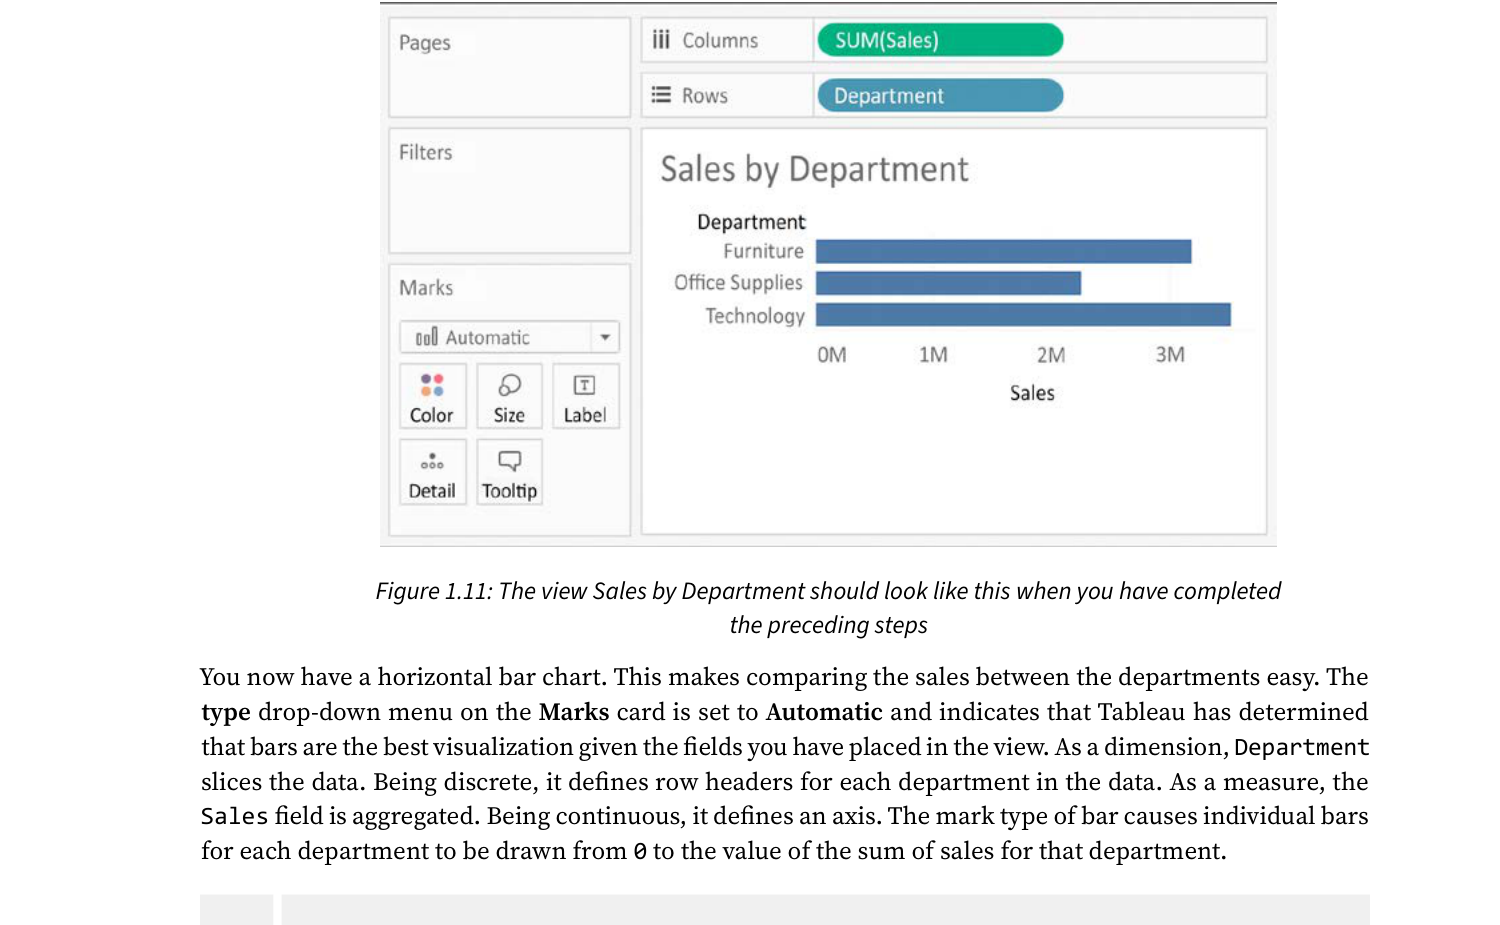
\includegraphics[width=0.9\linewidth]{images/bar_chart_basic.png}
\begin{figurecaptionmodern}
        \capfig{Bar Chart --- Sales by Department với Marks card hiển thị bên trái. \texttt{SUM(Sales)} trên Columns shelf, Department trên Rows shelf. Tableau tự chọn mark type = Automatic (bar).}
        \label{fig:bar_chart}
    \end{figurecaptionmodern}
\end{figure}

\noindent \textbf{Bước 3 --- Sắp xếp để dễ đọc hơn:} Nhấp vào biểu tượng \textbf{Sort Descending} trên toolbar (biểu tượng thanh cột A$\rightarrow$Z hoặc Z$\rightarrow$A) để sắp xếp từ doanh thu cao đến thấp. Biểu đồ đã sắp xếp luôn dễ đọc hơn --- người xem ngay lập tức thấy danh mục nào dẫn đầu mà không cần nhìn từng con số.

\noindent \textbf{Bước 4 --- Thêm màu theo Sub-Category (nâng cao):} Nếu muốn xem thêm phân rã theo danh mục con, kéo \textbf{\texttt{Sub-Category}} vào ô \textbf{Color} trong Marks card. Tableau tự động phân màu các điểm dữ liệu, biến biểu đồ thành \textbf{Stacked Bar Chart} --- mỗi cột được chia thành nhiều màu ứng với từng Sub-Category. Lúc này mỗi cột đại diện cho tổng doanh thu của một Category, các segment màu bên trong cho biết từng Sub-Category đóng góp bao nhiêu vào tổng đó.

\subsubsection{Biến thể nâng cao --- Stacked Bar Chart và Percent of Total}

\noindent Ngoài Stacked Bar Chart thông thường (giá trị tuyệt đối), một biến thể rất hữu ích là \textbf{Stacked Bar Chart 100\%} --- mỗi cột đều có chiều cao bằng nhau (= 100\%) và các segment màu thể hiện \textbf{tỷ lệ phần trăm} đóng góp của từng danh mục con. Loại biểu đồ này trả lời câu hỏi \textit{``Cơ cấu nội bộ của mỗi Category như thế nào?''} thay vì \textit{``Category nào bán được nhiều nhất?''}.

\noindent Để tạo Stacked Bar 100\%, sau khi đã có Stacked Bar Chart thông thường, thực hiện:

\noindent \textbf{Bước 5:} Nhấp chuột phải vào \texttt{SUM(Sales)} trên Rows shelf $\rightarrow$ chọn \textbf{Quick Table Calculation} $\rightarrow$ chọn \textbf{Percent of Total}. Tableau tính lại giá trị, mỗi segment bây giờ hiển thị tỷ lệ phần trăm thay vì giá trị tuyệt đối. Cần chỉ định \textbf{Compute Using} $\rightarrow$ \textbf{Cell} để Tableau hiểu tỷ lệ phần trăm được tính trong phạm vi mỗi Category (không phải toàn bộ dataset).

\noindent Kết quả: 3 cột với chiều cao bằng nhau, mỗi cột chia nhiều màu thể hiện tỷ trọng \% của từng Sub-Category trong từng Category --- cực kỳ hữu ích khi so sánh cơ cấu sản phẩm giữa các phân khúc thị trường.

\begin{guidelinebox}{Chuyển sang Horizontal Bar Chart}
Khi tên danh mục quá dài (ví dụ tên sản phẩm đầy đủ), biểu đồ cột đứng sẽ bị chồng chéo nhãn. Giải pháp: nhấp \textbf{Ctrl + W} (hoặc vào menu \textbf{Analysis $\rightarrow$ Swap Rows and Columns}) để đổi trục, biến thành Horizontal Bar Chart. Cột ngang thoải mái hơn cho tên dài và giúp mắt đọc từ trái sang phải tự nhiên hơn.
\end{guidelinebox}

\subsubsection{Sắp xếp (Sort) --- 4 phương pháp}

\noindent Sắp xếp biểu đồ từ cao đến thấp giúp người xem ngay lập tức thấy danh mục nào đứng đầu mà không cần quét qua toàn bộ biểu đồ. Tableau cung cấp 4 phương pháp sắp xếp khác nhau:

\noindent \textbf{Cách 1 --- Toolbar sort button:} Nhấp vào biểu tượng \textbf{Sort Ascending/Descending} trên toolbar. Đây là cách nhanh nhất --- Tableau tự động sắp xếp Dimension dựa trên Measure đang định nghĩa trục. Khi dữ liệu được cập nhật, thứ tự sắp xếp tự động cập nhật theo.

\noindent \textbf{Cách 2 --- Axis sort icon:} Di chuột lên trục số (trục X hoặc Y) --- một biểu tượng sắp xếp nhỏ xuất hiện cạnh tên trục. Nhấp vào đó để bật sắp xếp tự động --- kết quả giống Cách 1 nhưng kích hoạt từ trục thay vì toolbar.

\begin{figure}[H]
\centering
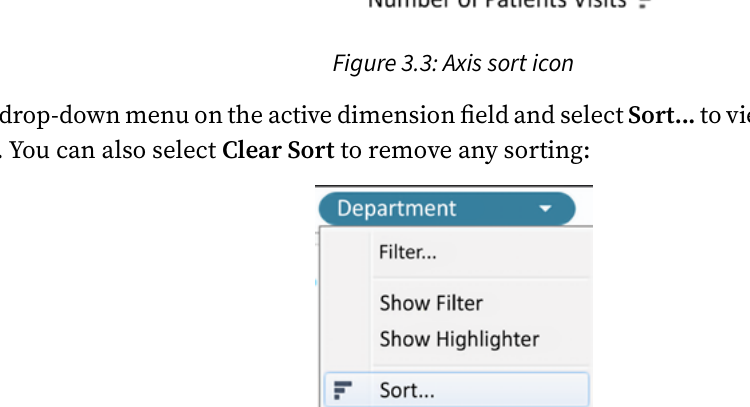
\includegraphics[width=0.7\linewidth]{images/sort_toolbar_icons.png}
\begin{figurecaptionmodern}
        \capfig{Axis sort icon --- biểu tượng sắp xếp xuất hiện trên trục khi di chuột.}
        \label{fig:sort_axis}
    \end{figurecaptionmodern}
\end{figure}

\noindent \textbf{Cách 3 --- Dropdown Sort menu:} Nhấp vào mũi tên bên cạnh tên Dimension trên header của biểu đồ --- menu drop-down xuất hiện với 4 kiểu sắp xếp:
\begin{itemize}[nosep]
    \item \textbf{Data source order} --- thứ tự trong file gốc
    \item \textbf{Alphabetic} --- sắp xếp theo bảng chữ cái
    \item \textbf{Field} --- sắp xếp theo Measure cụ thể (bạn chọn Measure nào)
    \item \textbf{Nested} --- sắp xếp riêng lẻ trong mỗi Panel (khi biểu đồ có nhiều panel)
\end{itemize}

\begin{figure}[H]
\centering
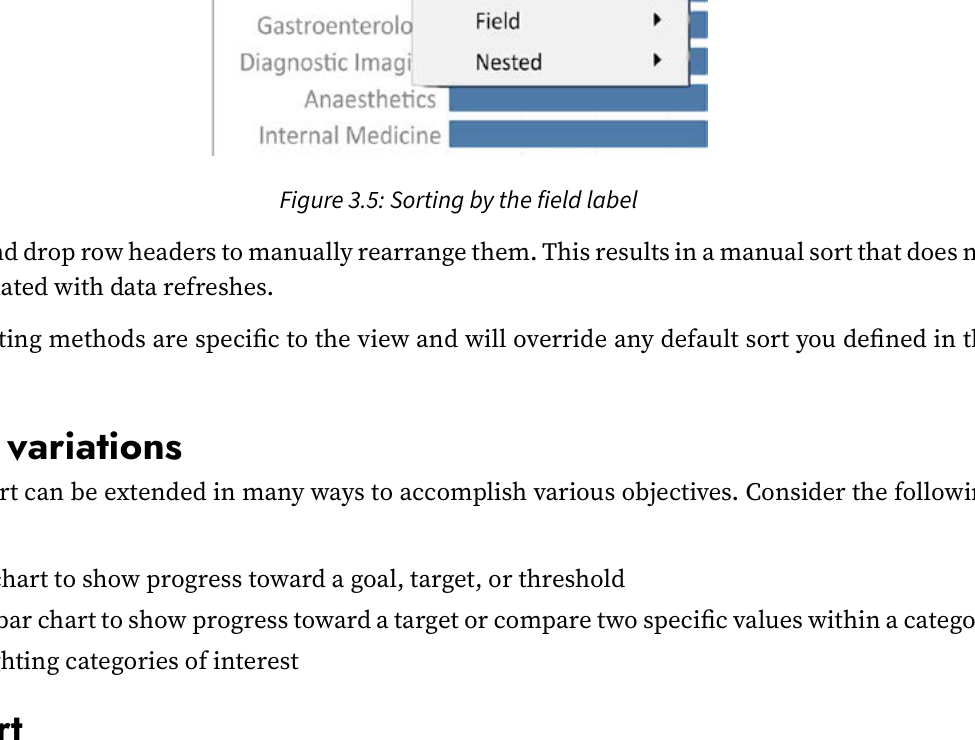
\includegraphics[width=0.7\linewidth]{images/sort_dropdown_menu.png}
\begin{figurecaptionmodern}
        \capfig{Dropdown Sort menu --- chọn Field hoặc Nested để sắp xếp theo Measure hoặc riêng từng Panel.}
        \label{fig:sort_dropdown}
    \end{figurecaptionmodern}
\end{figure}

\noindent \textbf{Cách 4 --- Kéo thủ công (Manual sort):} Giữ và kéo các header trên biểu đồ để sắp xếp thủ công. Kết quả là sắp xếp cố định (fixed) --- không tự cập nhật khi dữ liệu thay đổi. Đây là cách duy nhất để định nghĩa thứ tự tùy chỉnh (ví dụ: sắp xếp theo mức ưu tiên kinh doanh, không theo con số).

\begin{notebox}
Mọi phương pháp sắp xếp đều \textbf{ưu tiên theo view} và ghi đè lên thứ tự mặc định trong metadata. Khi sắp xếp không còn cần, nhấp chuột phải vào field $\rightarrow$ chọn \textbf{Clear Sort} để xóa.
\end{notebox}

\noindent \textbf{Tóm tắt Section II:} Chúng ta đã tạo Bar Chart cơ bản (Hình 1), tìm hiểu Stacked Bar và Percent of Total, và 4 phương pháp sắp xếp (Hình 2, 3).

% ===================================================================
\subsection{Line Chart --- Xu hướng theo thời gian}
% ===================================================================

\subsubsection{Khi nào dùng Line Chart?}

\noindent Line Chart (biểu đồ đường) là công cụ tối thượng để trả lời câu hỏi: \textbf{``Chỉ số này thay đổi như thế nào theo thời gian?''} Đường kẻ nối các điểm dữ liệu liên tiếp tạo ra một ``dòng chảy'' trực quan, giúp người xem tức thì nhận ra xu hướng tăng, giảm, hay dao động theo mùa. Đây là điều mà Bar Chart không thể làm tốt --- nếu trục X là 12 tháng liên tiếp cùng một biến, Bar Chart cho 12 cột rời rạc khó nhận ra xu hướng, trong khi Line Chart cho một đường rõ ràng.

\noindent Tuy nhiên, có một nguyên tắc quan trọng cần nhớ: \textbf{chỉ dùng Line Chart khi trục X là thời gian hoặc một dãy số có thứ tự liên tục}. Dùng Line Chart cho dữ liệu phân loại rời rạc (như 5 khu vực địa lý) là sai về mặt thống kê học --- đường nối giữa ``North'' và ``South'' không có ý nghĩa gì.

\subsubsection{Cách tạo Line Chart trong Tableau}

\noindent Chúng ta sẽ tạo biểu đồ theo dõi xu hướng doanh thu theo từng tháng trong Superstore.

\noindent \textbf{Bước 1:} Kéo field \textbf{\texttt{Order Date}} vào \textbf{Columns shelf}. Tableau nhận đây là Date field và tự động hiển thị \texttt{YEAR(Order Date)} --- tổng hợp theo năm. Bạn sẽ thấy trên biểu đồ các điểm dữ liệu rời rạc theo năm, chưa phải Line Chart.

\noindent \textbf{Bước 2:} Kéo field \textbf{\texttt{Sales}} vào \textbf{Rows shelf}. Lúc này Tableau đã có đủ thông tin: trục X là Date và trục Y là Measure số, nên tự động chuyển sang \textbf{Line Chart}.

\noindent \textbf{Bước 3 --- Drill down từ Năm xuống Tháng:} Hiện tại biểu đồ chỉ hiển thị theo năm --- quá thô để thấy xu hướng mùa vụ. Để xem chi tiết hơn, nhấp chuột phải vào \texttt{YEAR(Order Date)} đang hiển thị trên Columns shelf. Trong menu hiện ra, bạn thấy \textbf{2 nhóm tùy chọn} (tách biệt bởi đường kẻ ngang):
\begin{itemize}[nosep]
    \item Nhóm \textbf{trên} (xanh dương --- Discrete): trả về nhãn dạng header rời rạc
    \item Nhóm \textbf{dưới} (xanh lá --- Continuous): trả về trục liên tục theo thời gian
\end{itemize}

\noindent Chọn \textbf{\texttt{Month}} trong nhóm \textbf{dưới} (Continuous). Biểu đồ sẽ chuyển từ hiển thị theo năm sang theo từng tháng với trục thời gian liên tục, đường kẻ trở nên chi tiết và mượt hơn.

\begin{figure}[H]
\centering
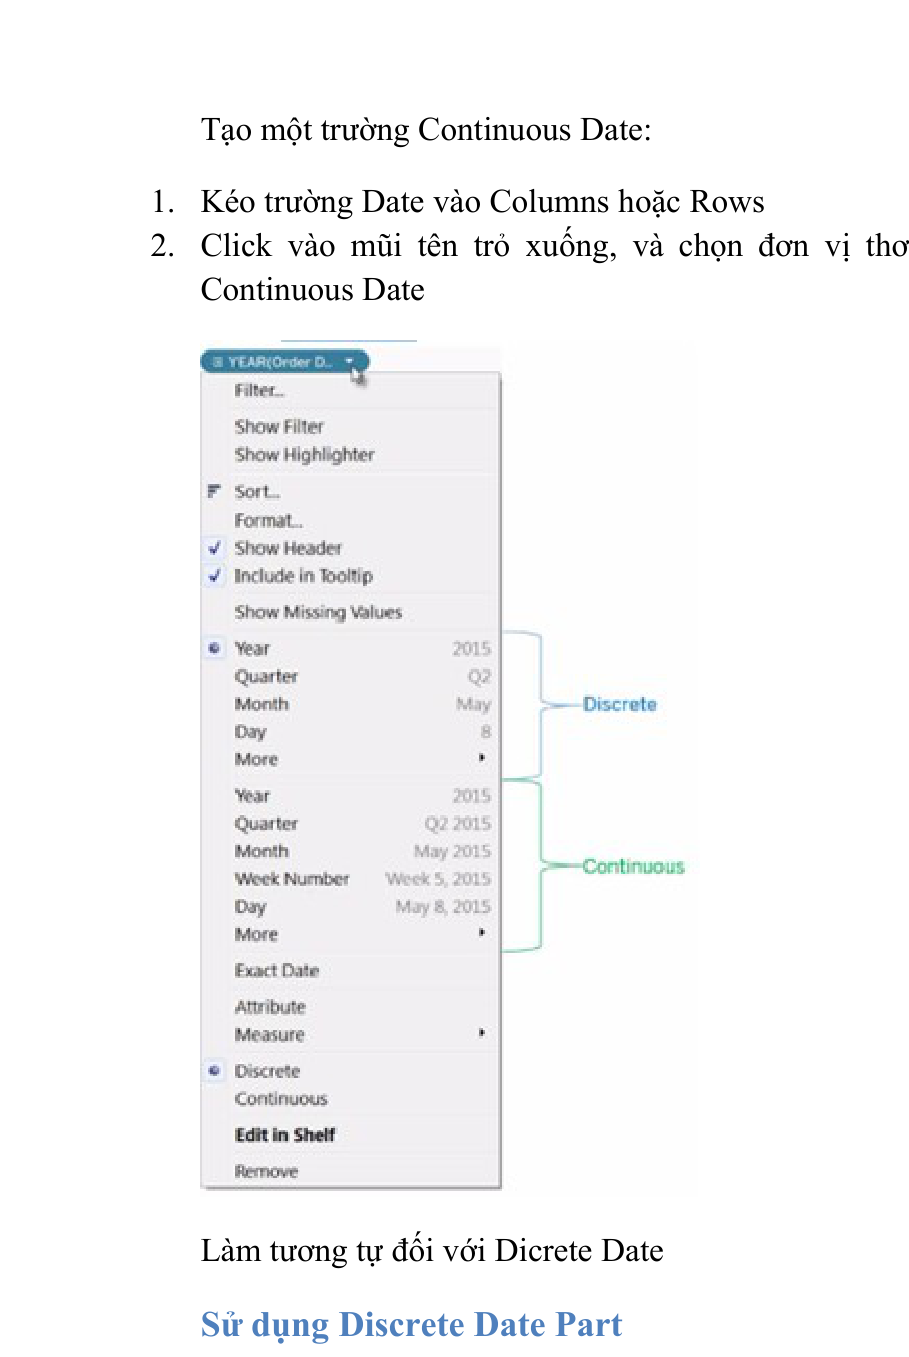
\includegraphics[width=0.7\linewidth]{images/discrete_continuous_date_menu.png}
\begin{figurecaptionmodern}
        \capfig{Menu chọn Discrete vs Continuous Date --- hai nhóm tùy chọn khi nhấp chuột phải vào Date pill. Nhóm trên (Discrete) tạo header rời rạc, nhóm dưới (Continuous) tạo trục liên tục.}
        \label{fig:date_menu}
    \end{figurecaptionmodern}
\end{figure}

\noindent \textbf{Bước 4 --- Thêm nhiều đường để so sánh:} Kéo \textbf{\texttt{Category}} vào ô \textbf{Color} trong Marks card. Tableau sẽ vẽ \textbf{3 đường riêng biệt} --- một đường cho mỗi Category, phân biệt bằng màu sắc. Bây giờ chúng ta có thể so sánh xu hướng doanh thu của Furniture vs Office Supplies vs Technology theo cùng trục thời gian.

\begin{guidelinebox}{Discrete Date vs Continuous Date: khác nhau quan trọng}
Khi nhấp chuột phải vào một Date field trên shelf, Tableau luôn hiển thị 2 nhóm lựa chọn:
\begin{itemize}[nosep]
    \item \textbf{Discrete (màu xanh dương):} Mỗi giá trị thời gian trở thành một \textbf{header riêng biệt}. Ví dụ ``January'', ``February''... hoặc ``2021'', ``2022''... --- hữu ích khi muốn tạo cột riêng theo năm trong bảng.
    \item \textbf{Continuous (màu xanh lá):} Thời gian được hiểu là một \textbf{trục liên tục} --- đường kẻ chạy mượt, tỷ lệ giữa các điểm thời gian được bảo toàn chính xác.
\end{itemize}
\textbf{Quy tắc:} Với Line Chart, \textbf{luôn} chọn Continuous để trục X phản ánh đúng dòng chảy thời gian. Dùng Discrete chỉ khi muốn tạo các cột tiêu đề tách biệt (như trong Text Table theo năm).
\end{guidelinebox}

\begin{figure}[H]
\centering
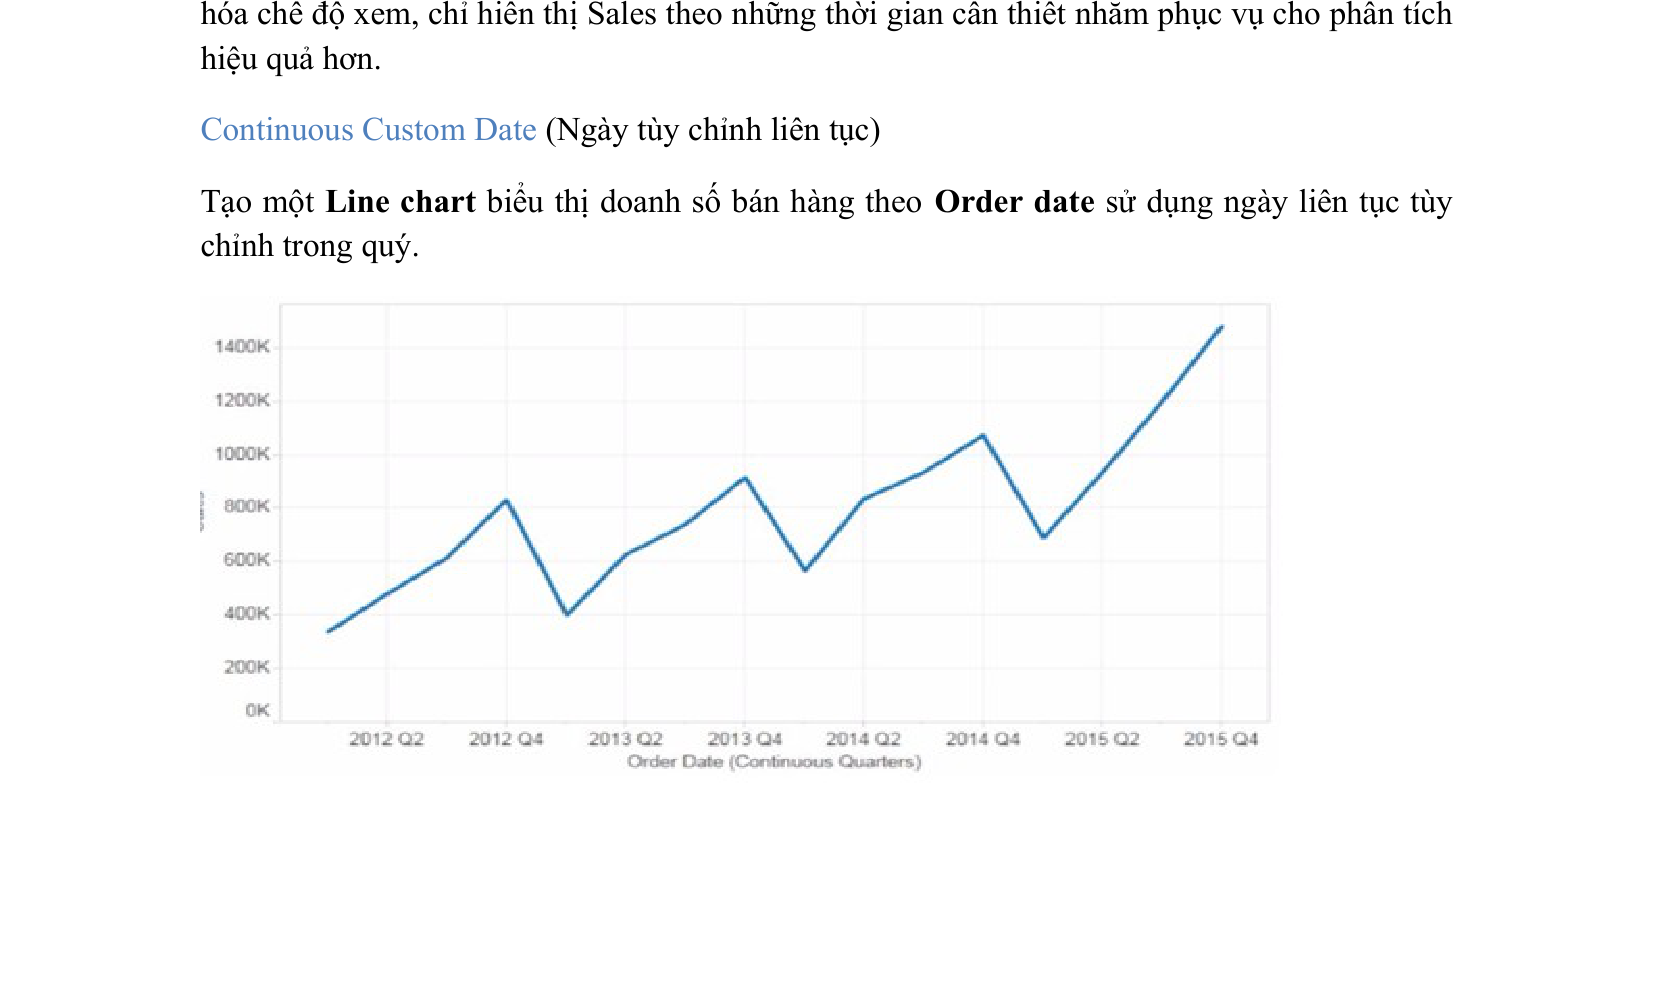
\includegraphics[width=0.9\linewidth]{images/line_chart_continuous.png}
\begin{figurecaptionmodern}
        \capfig{Line Chart --- Doanh thu theo Order Date (Continuous Quarters). Đường kẻ nối liền mạch từ 2012 Q2 đến 2015 Q4, cho thấy xu hướng doanh thu tăng rõ rệt.}
        \label{fig:line_chart}
    \end{figurecaptionmodern}
\end{figure}

\subsubsection{Discrete vs Continuous Date --- Hiểu sâu để tạo biểu đồ đúng}

\noindent Đây là một trong những concept quan trọng nhất khi làm việc với dữ liệu thời gian trong Tableau, và cũng là nguồn gốc của rất nhiều lỗi biểu đồ khó hiểu: \textbf{tại sao đường kẻ bị đứt khi qua năm mới?}

\begin{center}
\renewcommand{\arraystretch}{1.4}
\begin{tabularx}{\linewidth}{X X}
\toprule
\textbf{Discrete Date (xanh dương)} & \textbf{Continuous Date (xanh lá)} \\
\midrule
Mỗi giá trị = một \textbf{header riêng biệt} & Toàn bộ = một \textbf{trục số liên tục} \\
\texttt{YEAR(Date)} Discrete: \texttt{2022 | 2023 | 2024} riêng biệt & \texttt{YEAR(Date)} Continuous: trục 2022$\rightarrow$2024 liền mạch \\
Pill \textbf{màu xanh dương} trên shelf & Pill \textbf{màu xanh lá} trên shelf \\
\texttt{MONTH(Date)} Discrete: Jan$\rightarrow$Dec cho mỗi năm & \texttt{MONTH(Date)} Continuous: DATE value bị truncate theo tháng \\
Đường \textbf{không nối qua} giữa các năm & Đường \textbf{nối liền} xuyên suốt các năm \\
\bottomrule
\end{tabularx}
\end{center}

\noindent \textbf{Ví dụ minh họa --- Tại sao đường bị đứt:}

\noindent Nếu bạn kéo \texttt{Order Date} vào Columns shelf và chọn \texttt{Month} (Discrete, màu xanh dương), Tableau tạo ra 12 header \textbf{January, February, ..., December} --- mỗi năm tạo \textbf{một bộ 12 header riêng} và đường không nối qua giữa năm. Đây là Discrete --- nó hỏi ``tháng 1 năm nào?'' chứ không biết thứ tự giữa các năm.

\noindent Nếu chọn \texttt{MONTH(Date)} Continuous (màu xanh lá), Tableau tạo một \textbf{trục Date liên tục} từ January 2021 $\rightarrow$ December 2024 liền mạch, đường kẻ nối thông suốt qua các năm.

\noindent \textbf{Cách chuyển đổi:} Nhấp chuột phải vào Date pill đang hiển thị trên shelf $\rightarrow$ menu xuất hiện với \textbf{2 nhóm tùy chọn} (nhóm trên = Discrete xanh dương, nhóm dưới = Continuous xanh lá):
\begin{itemize}[nosep]
    \item Chọn cùng cấp độ (Year/Quarter/Month) ở nhóm Continuous để chuyển từ Discrete sang Continuous
    \item Hoặc nhấp chuột phải vào pill $\rightarrow$ chọn ``Discrete'' / ``Continuous'' trực tiếp
\end{itemize}

\begin{notebox}
\textbf{Quy tắc đơn giản:}
\begin{itemize}[nosep]
    \item Dùng Line Chart để xem xu hướng theo thời gian $\rightarrow$ luôn chọn \textbf{Continuous date}
    \item Dùng Discrete date khi cần tạo header riêng biệt (như trong Text Table theo năm-tháng)
    \item Nếu đường bị đứt, kiểm tra ngay: pill Date có màu xanh dương không? Nếu có, hãy chuyển sang Continuous.
\end{itemize}
\end{notebox}

% ===================================================================
\subsection{Area Chart --- Nhấn mạnh khối lượng tích lũy theo thời gian}
% ===================================================================

\subsubsection{Khi nào dùng Area Chart?}

\noindent Area Chart thực chất là \textbf{Line Chart với vùng dưới đường được tô màu}. Sự khác biệt tuy đơn giản nhưng mang ý nghĩa truyền thông quan trọng: Line Chart nhấn mạnh \textbf{xu hướng} (lên hay xuống), còn Area Chart nhấn mạnh \textbf{khối lượng tích lũy} (tổng giá trị qua thời gian). Hãy tưởng tượng Line Chart như đường chân trời --- bạn thấy hướng đi nhưng không thấy ``lượng'' bên dưới. Area Chart lấp đầy phần đó.

\noindent Dùng Area Chart khi:
\begin{itemize}[nosep]
    \item Muốn thể hiện \textbf{phần đóng góp của từng nhóm} trong tổng giá trị theo thời gian (Stacked Area)
    \item Muốn nhấn mạnh \textbf{khối lượng tổng cộng} chứ không chỉ đường xu hướng
    \item Có 2--4 nhóm cần so sánh --- quá nhiều nhóm sẽ khiến biểu đồ trở nên rối và khó đọc
\end{itemize}

\subsubsection{Cách tạo Area Chart trong Tableau}

\noindent \textbf{Bước 1:} Kéo \textbf{\texttt{Order Date}} vào \textbf{Columns shelf}. Nhấp chuột phải $\rightarrow$ chọn \textbf{Month} (Continuous) trong nhóm dưới để có trục thời gian liên tục.

\noindent \textbf{Bước 2:} Kéo \textbf{\texttt{Sales}} vào \textbf{Rows shelf}. Tableau tạo Line Chart mặc định.

\noindent \textbf{Bước 3 --- Chuyển sang Area Chart:} Trong \textbf{Marks card}, nhấp vào dropdown \textbf{Mark Type} (đang hiển thị ``Automatic'' hoặc ``Line'') $\rightarrow$ chọn \textbf{Area}. Vùng dưới đường kẻ lập tức được tô màu --- biểu đồ bây giờ nhấn mạnh tổng khối lượng bán hàng tích lũy.

\noindent \textbf{Bước 4 --- Tạo Stacked Area Chart:} Kéo \textbf{\texttt{Category}} vào ô \textbf{Color} trong Marks card. Tableau tạo 3 vùng màu xếp chồng (stacked) --- Furniture, Office Supplies, Technology. Mỗi vùng thể hiện phần đóng góp của Category đó vào tổng doanh thu. Vùng phía trên cùng chính là tổng doanh thu toàn công ty.

\begin{guidelinebox}{Area Chart vs Line Chart: khi nào chọn cái nào?}
\renewcommand{\arraystretch}{1.3}
\begin{tabularx}{\linewidth}{l X X}
\toprule
\textbf{Tiêu chí} & \textbf{Line Chart} & \textbf{Area Chart} \\
\midrule
Mục đích chính & Xu hướng & Khối lượng / tỷ trọng \\
Nhiều nhóm & Dễ đọc (đường tách biệt) & Khó đọc nếu > 4 nhóm (vùng chồng lấp) \\
Giá trị âm & Hiển thị tốt & Khó diễn giải khi tô màu vùng âm \\
Stacked & Không hỗ trợ & Mạnh --- thể hiện phần đóng góp \\
\bottomrule
\end{tabularx}

\noindent \textbf{Quy tắc nhanh:} Nếu chỉ cần xem xu hướng $\rightarrow$ Line. Nếu muốn thấy ``miếng bánh'' thay đổi theo thời gian $\rightarrow$ Stacked Area.
\end{guidelinebox}

\begin{notebox}
\textbf{Cạm bẫy --- Stacked Area có thể gây hiểu lầm.} Trong Stacked Area, vùng trên cùng bị ``đẩy lên'' bởi các vùng bên dưới. Điều này có nghĩa \textbf{đường biên trên của một vùng KHÔNG phải là giá trị thực} của nhóm đó --- nó là tổng tích lũy. Nếu người đọc không hiểu điều này, họ sẽ đánh giá sai kích thước vùng trên cùng. Giải pháp: dùng \textbf{Percent of Total Stacked Area} (nhấp chuột phải vào \texttt{SUM(Sales)} $\rightarrow$ Quick Table Calculation $\rightarrow$ Percent of Total) khi muốn so sánh tỷ trọng thay vì giá trị tuyệt đối.
\end{notebox}

% ===================================================================
\subsection{Scatter Plot --- Khám phá tương quan giữa hai chỉ số}
% ===================================================================

\subsubsection{Khi nào dùng Scatter Plot?}

\noindent Scatter Plot (biểu đồ phân tán) là công cụ lý tưởng để trả lời câu hỏi: \textbf{``Hai chỉ số này có liên quan với nhau không?''} Mỗi điểm trên Scatter Plot đại diện cho một đơn thể (sản phẩm, khách hàng, đơn hàng...) với vị trí trên trục X xác định bởi chỉ số thứ nhất và trục Y bởi chỉ số thứ hai. Nếu các điểm tập trung theo một đường chéo từ dưới-trái lên trên-phải, hai chỉ số có \textbf{tương quan thuận} (cái này tăng thì cái kia cũng tăng). Nếu ngược lại, chúng có \textbf{tương quan nghịch}.

\noindent Trong ngữ cảnh Superstore, Scatter Plot giúp trả lời những câu hỏi kinh doanh quan trọng: Các sản phẩm bán nhiều (\texttt{Sales} cao) có mang lại lợi nhuận cao (\texttt{Profit} cao) không? Hay có những sản phẩm ``bán chạy nhưng lỗ'' mà ta cần loại bỏ? Ngoài ra, Scatter Plot cũng giỏi phát hiện \textbf{outliers} --- những điểm nằm xa đám mây điểm chính, có thể là cơ hội hoặc vấn đề cần điều tra.

\subsubsection{Cách tạo Scatter Plot trong Tableau}

\noindent \textbf{Bước 1:} Kéo \textbf{\texttt{Sales}} (Measure) vào \textbf{Columns shelf} --- đây sẽ là trục X.

\noindent \textbf{Bước 2:} Kéo \textbf{\texttt{Profit}} (Measure) vào \textbf{Rows shelf} --- đây sẽ là trục Y.

\noindent Ngay lúc này, Tableau hiển thị \textbf{chỉ 1 điểm duy nhất} ở giữa canvas. Đừng bối rối --- đây không phải lỗi. Tableau đang hiển thị \texttt{SUM(Sales)} và \texttt{SUM(Profit)} của \textbf{toàn bộ dataset} gộp lại thành một con số tổng, nên chỉ có 1 điểm. Biểu đồ này chưa có ý nghĩa phân tích.

\noindent \textbf{Bước 3 --- Bước quan trọng nhất:} Kéo \textbf{\texttt{Sub-Category}} vào ô \textbf{Detail} trong Marks card. Tableau hiểu rằng bây giờ chúng ta muốn nhìn từng \textbf{Sub-Category riêng} thay vì tổng hợp tất cả. Ngay lập tức, 1 điểm biến thành \textbf{17 điểm} --- mỗi điểm là một Sub-Category với tọa độ \texttt{(SUM(Sales), SUM(Profit))} của riêng nó.

\noindent \textbf{Bước 4 --- Thêm màu và kích thước:} Kéo \textbf{\texttt{Category}} vào \textbf{Color} để phân biệt 3 nhóm lớn bằng màu. Kéo \textbf{\texttt{Quantity}} vào \textbf{Size} để kích thước điểm phản ánh số lượng bán ra --- điểm to = bán nhiều đơn. Lúc này mỗi điểm mang 4 chiều thông tin: Sales (trục X), Profit (trục Y), Category (màu), Quantity (kích thước).

\noindent \textbf{Bước 5 --- Thêm tứ phân vị (nâng cao):} Vào menu \textbf{Analysis $\rightarrow$ Add Reference Line}. Chọn \textbf{Average} cho trục X và tương tự cho trục Y. Hai đường trung bình tạo thành 4 góc phần tư (quadrant) giúp phân loại các Sub-Category:
\begin{itemize}[nosep]
    \item Góc trên-phải: Sales cao + Profit cao $\rightarrow$ \textbf{``Stars''} (giữ và đầu tư)
    \item Góc dưới-phải: Sales cao + Profit thấp $\rightarrow$ \textbf{``Cash Cows''} (bán nhiều nhưng lãi ít --- cần xem xét giá)
    \item Góc trên-trái: Sales thấp + Profit cao $\rightarrow$ \textbf{``Niche''} (lãi tốt nhưng ít bán --- tìm cách mở rộng)
    \item Góc dưới-trái: Sales thấp + Profit thấp $\rightarrow$ \textbf{``Question Marks''} (cân nhắc loại bỏ)
\end{itemize}

\subsubsection{Đọc hiểu kết quả --- 3 loại tương quan và Outliers}

\noindent Khi phân tích Scatter Plot, kỹ năng quan trọng nhất là nhận ra \textbf{kiểu phân bố của đám mây điểm} và từ đó suy ra mối quan hệ giữa hai biến:

\begin{center}
\renewcommand{\arraystretch}{1.4}
\begin{tabularx}{\linewidth}{>{\raggedright\arraybackslash}p{3cm} X X}
\toprule
\textbf{Loại tương quan} & \textbf{Mô tả đám mây điểm} & \textbf{Ý nghĩa} \\
\midrule
\textbf{Positive} & Điểm từ dưới-trái lên trên-phải & Một biến tăng $\rightarrow$ biến kia cũng tăng. VD: Sales tăng đi cùng Profit tăng \\
\textbf{Negative} & Điểm từ trên-trái xuống dưới-phải & Một biến tăng $\rightarrow$ biến kia giảm. VD: Discount cao đi cùng Profit thấp \\
\textbf{No relation} & Điểm rải đều không theo hướng nào & Hai biến độc lập nhau \\
\bottomrule
\end{tabularx}
\end{center}

\noindent Ngoài ba nhóm trên, cần chú ý đặc biệt đến \textbf{Outliers} --- những điểm nằm cô lập xa đám mây điểm chính. Trong Superstore, một Sub-Category có Profit âm lớn trong khi phần còn lại đều dương chính là outlier --- đây là tín hiệu cần điều tra: giá bán quá thấp? Chi phí vận chuyển quá cao? Chính sách chiết khấu không phù hợp?

\noindent Tableau cung cấp 2 cách xử lý Outliers trực tiếp trên biểu đồ:
\begin{itemize}[nosep]
    \item \textbf{Annotate (Chú thích):} Nhấp chuột phải vào điểm outlier $\rightarrow$ \textbf{Annotate $\rightarrow$ Mark} $\rightarrow$ nhập mô tả. Chú thích này xuất hiện ngay trên biểu đồ, hữu ích khi trình bày để đánh dấu Sub-Category cần chú ý.
    \item \textbf{Exclude (Loại trừ tạm thời):} Nhấp chuột phải vào điểm outlier $\rightarrow$ \textbf{Exclude}. Điểm bị ẩn khỏi view để phần còn lại hiển thị với scale phù hợp hơn. Lưu ý đây chỉ là ẩn hiển thị --- dữ liệu gốc không bị xóa và Tableau sẽ thông báo rõ ``1 member is excluded''.
\end{itemize}

\subsubsection{Công cụ phân tích nâng cao --- Highlighter}

\noindent Khi Scatter Plot có nhiều điểm dữ liệu (hàng chục Sub-Category hoặc hàng trăm sản phẩm), rất khó nhìn ra một điểm cụ thể giữa đám mây. \textbf{Highlighter} là giải pháp: nó cho phép gõ tên để tô sáng tức thì các điểm liên quan trong khi làm mờ phần còn lại, giúp so sánh ad-hoc một cách trực quan.

\noindent Cách bật Highlighter: Nhấp chuột phải vào một Dimension field trong Marks card $\rightarrow$ chọn \textbf{Show Highlighter}. Một ô tìm kiếm nhỏ xuất hiện góc trên bên phải của biểu đồ. Khi bạn gõ, các điểm khớp với tìm kiếm sẽ được tô sáng ngay lập tức --- ví dụ gõ ``Chairs'' sẽ làm nổi bật toàn bộ điểm thuộc Sub-Category Chairs trong tất cả các chart trên dashboard.

\begin{notebox}
\textbf{Tại sao Scatter Plot chỉ hiện 1 điểm?} --- Đây là điểm gây nhầm lẫn phổ biến nhất với Scatter Plot trong Tableau. Khi bạn đặt 2 Measure vào Rows và Columns mà \textbf{không có bất kỳ Dimension nào trong Detail, Color, hay Shape}, Tableau tổng hợp (aggregate) tất cả dữ liệu thành \textbf{một cụm điểm duy nhất} --- tổng Sales và tổng Profit của toàn bộ dataset.

\noindent \textbf{Giải pháp:} Kéo \textbf{ít nhất 1 Dimension} vào ô \textbf{Detail} hoặc \textbf{Color} trong Marks card. Dimension này sẽ ``phá vỡ'' sự tổng hợp và tạo ra một điểm riêng cho mỗi giá trị của Dimension đó. Quy tắc này áp dụng cho mọi biểu đồ sử dụng 2 Measure trên 2 trục.
\end{notebox}

\begin{figure}[H]
\centering
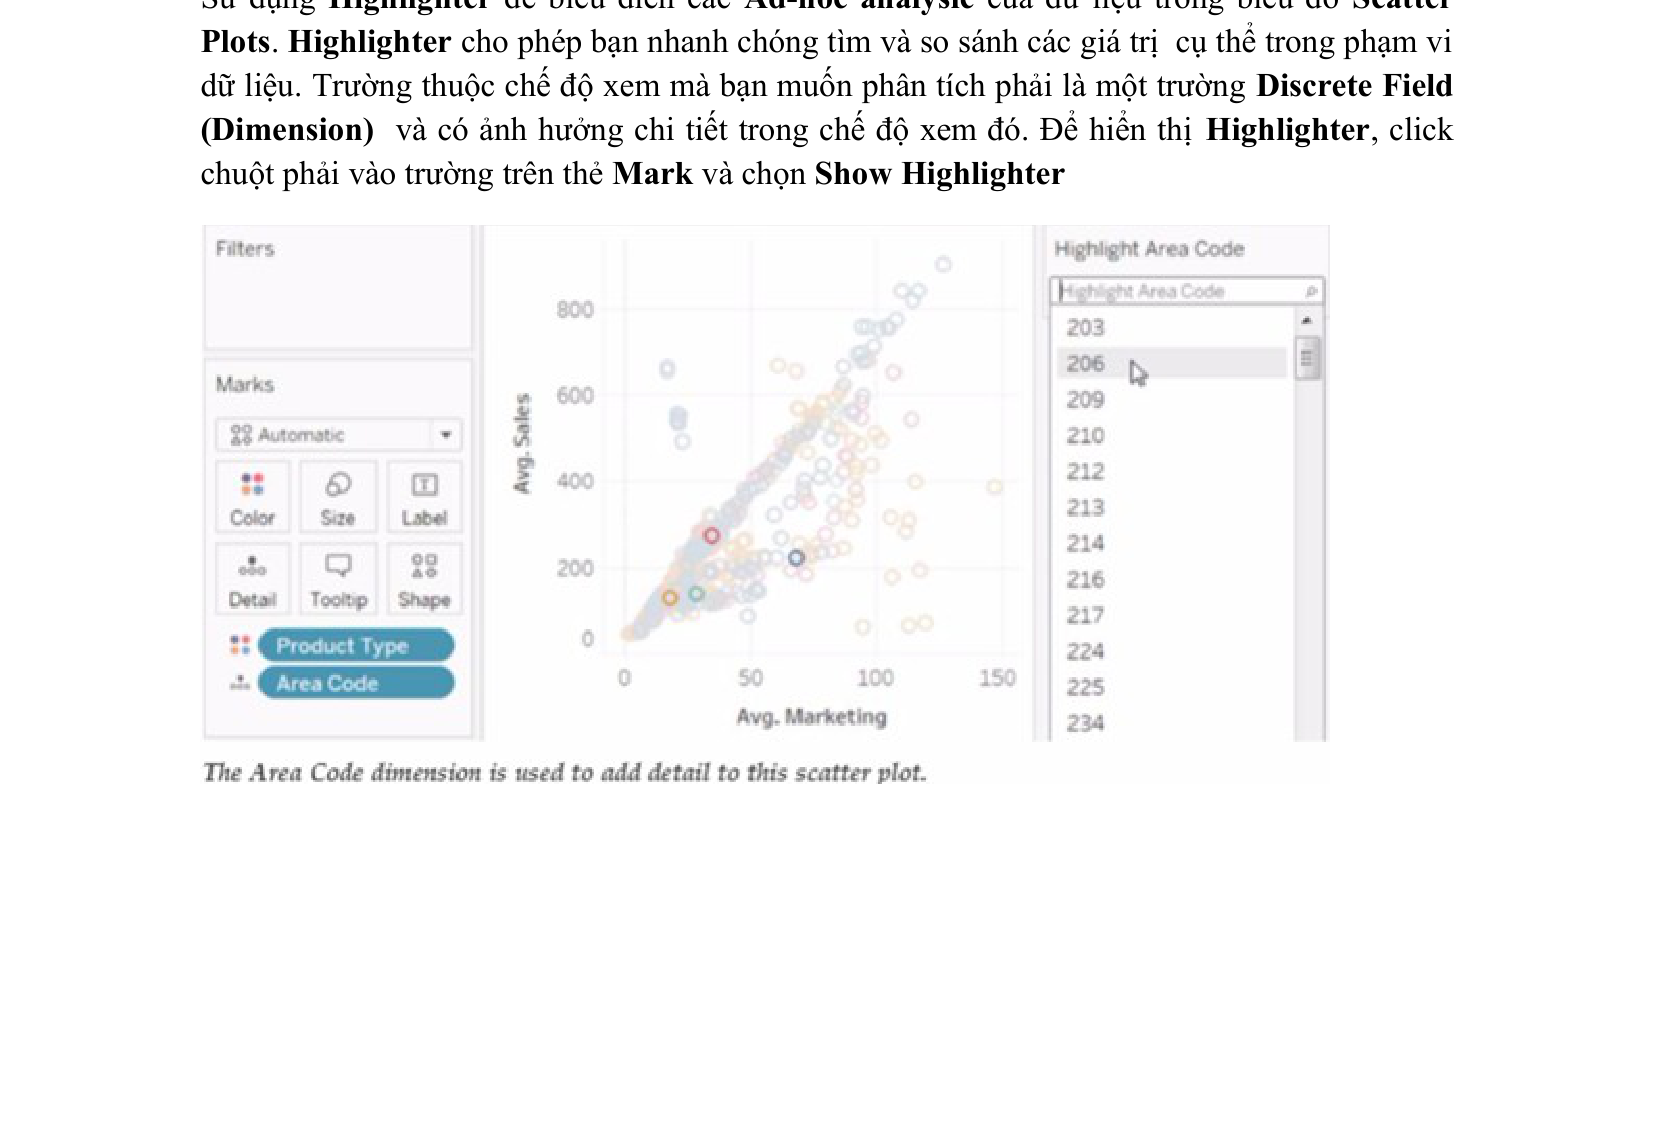
\includegraphics[width=0.9\linewidth]{images/scatter_plot_highlighter.png}
\begin{figurecaptionmodern}
        \capfig{Scatter Plot với Highlighter panel --- mỗi điểm đại diện cho một Area Code, màu phân biệt theo Product Type. Dimension ``Area Code'' được kéo vào Detail trong Marks card để tạo nhiều điểm thay vì 1 điểm tổng hợp.}
        \label{fig:scatter_plot}
    \end{figurecaptionmodern}
\end{figure}

% ===================================================================
\subsection{Histogram --- Xem phân phối của dữ liệu}
% ===================================================================

\subsubsection{Khi nào dùng Histogram?}

\noindent Histogram trả lời câu hỏi: \textit{``Dữ liệu phân bố như thế nào?''} --- đa số đơn hàng rơi vào khoảng giá nào? Có bao nhiêu kích thước đơn hàng rất lớn so với trung bình? \textbf{Histogram trông giống Bar Chart nhưng khác biệt cơ bản}: Bar Chart so sánh giữa các \textbf{danh mục rời rạc} (Furniture vs Technology), còn Histogram chia một \textbf{biến liên tục} thành các khoảng (bins) và đếm số lượng rơi vào từng khoảng.

\noindent Dùng Histogram khi:
\begin{itemize}[nosep]
    \item Muốn hiểu hình dạng phân phối của dữ liệu (chuông, lệch phải, đa đỉnh...)
    \item Muốn nhận ra \textbf{outlier} (giá trị bất thường) một cách trực quan
    \item Muốn biết \textbf{đa số} dữ liệu rơi vào khoảng nào (VD: đa số đơn hàng Superstore có giá \$0--\$500)
\end{itemize}

\subsubsection{Cách tạo Histogram trong Tableau}

\noindent \textbf{Cách 1 --- Dùng Show Me (nhanh nhất):}
\begin{enumerate}[nosep]
    \item Trong Data Pane, nhấp chọn field \textbf{\texttt{Sales}} (hoặc bất kỳ Measure nào muốn xem phân phối).
    \item Nhấp \textbf{Show Me} (góc trên bên phải) $\rightarrow$ chọn biểu tượng \textbf{Histogram} (hình các cột liền kề nhau). Tableau tự động tạo \textbf{Bin} và hiển thị Histogram hoàn chỉnh.
\end{enumerate}

\noindent \textbf{Cách 2 --- Tạo thủ công (kiểm soát bin size):}
\begin{enumerate}[nosep]
    \item Trong Data Pane, nhấp chuột phải vào \textbf{\texttt{Sales}} $\rightarrow$ \textbf{Create $\rightarrow$ Bins...}
    \item Tableau gợi ý \textbf{Bin Size} tự động (dựa trên range của dữ liệu). Bạn có thể chỉnh --- ví dụ: đặt Bin Size = \textbf{200} nghĩa là mỗi cột đại diện cho khoảng \$200 (0--200, 200--400, 400--600...). Nhấp \textbf{OK}.
    \item Trong Data Pane xuất hiện field mới \textbf{\texttt{Sales (bin)}} (icon giống Dimension kèm ký hiệu bin). Kéo \textbf{\texttt{Sales (bin)}} vào \textbf{Columns shelf}.
    \item Kéo \textbf{\texttt{Sales}} vào \textbf{Rows shelf} $\rightarrow$ nhấp chuột phải $\rightarrow$ chọn \textbf{Measure (Count)} hoặc \textbf{CNT(Sales)}. Lúc này Histogram hoàn chỉnh: trục X là khoảng giá, trục Y là số lượng đơn hàng.
\end{enumerate}

\begin{guidelinebox}{Chọn Bin Size phù hợp}
Bin Size quá nhỏ $\rightarrow$ biểu đồ rối, khó thấy pattern. Bin Size quá lớn $\rightarrow$ mất chi tiết, mọi thứ dồn vào 2--3 cột. Quy tắc thực tế: bắt đầu với Bin Size mặc định của Tableau, sau đó thử tăng/giảm để tìm mức hiển thị rõ nhất hình dạng phân phối. Để chỉnh lại: nhấp chuột phải vào \textbf{\texttt{Sales (bin)}} trong Data Pane $\rightarrow$ \textbf{Edit...}
\end{guidelinebox}

\begin{notebox}
\textbf{Khác biệt Bar Chart vs Histogram:}
\renewcommand{\arraystretch}{1.3}
\begin{tabularx}{\linewidth}{l X X}
\toprule
& \textbf{Bar Chart} & \textbf{Histogram} \\
\midrule
Trục X & Danh mục rời rạc (Category) & Khoảng liên tục (Bins) \\
Khoảng cách cột & Có gap giữa các cột & Không có gap (liền kề) \\
Ý nghĩa & So sánh giá trị giữa nhóm & Phân phối / tần suất \\
\bottomrule
\end{tabularx}
\end{notebox}

% ===================================================================
\subsection{Box Plot (Box \& Whisker) --- So sánh phân phối giữa các nhóm}
% ===================================================================

\subsubsection{Khi nào dùng Box Plot?}

\noindent Box Plot (đôi khi gọi là Box \& Whisker) là công cụ thống kê chuyên dụng để \textbf{so sánh phân phối của một Measure giữa nhiều nhóm} --- ví dụ: mức Discount trung bình và độ biến động giữa các Region khác nhau như thế nào? Box Plot nén 5 thông tin thống kê vào 1 hình: \textbf{trung vị (median)}, \textbf{tứ phân vị 1 và 3 (Q1, Q3)}, \textbf{râu (whiskers)}, và \textbf{outlier}.

\noindent Dùng Box Plot khi:
\begin{itemize}[nosep]
    \item Muốn so sánh \textbf{độ phân tán} của dữ liệu giữa nhiều nhóm (VD: Profit distribution theo Category)
    \item Muốn nhận ra \textbf{outlier} (giá trị nằm ngoài râu) --- các điểm bất thường cần điều tra
    \item Muốn biết \textbf{giá trị điển hình} (median) và \textbf{độ biến động} (IQR = Q3 -- Q1) của mỗi nhóm
\end{itemize}

\subsubsection{Cách tạo Box Plot trong Tableau}

\noindent \textbf{Bước 1:} Kéo \textbf{\texttt{Region}} (Dimension) vào \textbf{Columns shelf} --- tạo các nhóm để so sánh.

\noindent \textbf{Bước 2:} Kéo \textbf{\texttt{Discount}} (Measure) vào \textbf{Rows shelf}. Tableau mặc định tạo Bar Chart với \texttt{SUM(Discount)} --- chưa đúng.

\noindent \textbf{Bước 3 --- Tăng độ chi tiết:} Kéo \textbf{\texttt{Sub-Category}} (hoặc bất kỳ Dimension nào có nhiều giá trị) vào ô \textbf{Detail} trong Marks card. Điều này ``phá vỡ'' sự tổng hợp --- mỗi Sub-Category trở thành một điểm dữ liệu riêng.

\noindent \textbf{Bước 4 --- Chuyển sang Box Plot:} Nhấp \textbf{Show Me} $\rightarrow$ chọn \textbf{Box-and-Whisker Plot}. Tableau tự động tính toán median, Q1/Q3, và vẽ râu + outlier.

\subsubsection{Đọc hiểu Box Plot}

\begin{center}
\renewcommand{\arraystretch}{1.4}
\begin{tabularx}{\linewidth}{l X}
\toprule
\textbf{Thành phần} & \textbf{Ý nghĩa} \\
\midrule
Đường nằm ngang trong hộp & \textbf{Median} --- giá trị trung vị (50\% dữ liệu trên, 50\% dưới) \\
Cạnh dưới hộp & \textbf{Q1} (Quartile 1) --- 25\% dữ liệu nằm dưới mức này \\
Cạnh trên hộp & \textbf{Q3} (Quartile 3) --- 75\% dữ liệu nằm dưới mức này \\
Chiều cao hộp (IQR) & \textbf{Q3 -- Q1} --- càng cao = dữ liệu càng phân tán \\
Râu (whiskers) & Mở rộng đến giá trị xa nhất trong khoảng 1.5 $\times$ IQR \\
Điểm riêng lẻ (outlier) & Giá trị nằm ngoài râu --- \textbf{bất thường}, cần điều tra \\
\bottomrule
\end{tabularx}
\end{center}

\begin{guidelinebox}{Tùy chỉnh hiển thị outlier}
Mặc định Tableau hiển thị outlier như các điểm tròn nhỏ. Để tùy chỉnh: nhấp chuột phải vào trục Y $\rightarrow$ \textbf{Edit Reference Line} $\rightarrow$ thay đổi \textbf{Whisker} và \textbf{Outlier} style. Bạn có thể ẩn outlier hoặc đổi màu để nhấn mạnh.
\end{guidelinebox}

% ===================================================================
\subsection{Text Table, Heat Map \& Highlight Table --- Bảng số liệu và màu sắc}
% ===================================================================

\subsubsection{Khi nào dùng Text Table?}

\noindent Text Table (còn được gọi là Crosstab --- bảng chéo, hay Pivot Table) là biểu đồ theo nghĩa rộng nhất: nó không vẽ hình, mà hiển thị \textbf{con số cụ thể trong từng ô giao nhau} của hàng và cột. Đây là lựa chọn phù hợp khi người đọc cần \textbf{tra cứu hoặc so sánh giá trị chính xác} --- ``Doanh thu của Furniture trong năm 2023 là bao nhiêu đúng?'' là câu hỏi mà Bar Chart hay Line Chart không trả lời được trực tiếp, nhưng Text Table thì có.

\noindent Tuy nhiên, Text Table cũng có nhược điểm đáng kể: rất khó nhận ra xu hướng, khó so sánh giữa nhiều con số cùng lúc, và trở nên khó đọc khi có nhiều hàng/cột. Một quy tắc thực tế: \textbf{chỉ dùng Text Table khi người xem thực sự cần con số chính xác} --- ví dụ báo cáo tài chính, bảng KPI hàng tháng, hay khi người đọc là kế toán cần đối chiếu số liệu. Với hầu hết mục đích trình bày và phân tích xu hướng, các loại biểu đồ trực quan (Bar, Line, Area, Scatter...) sẽ hiệu quả hơn.

\subsubsection{Cách tạo Text Table trong Tableau}

\noindent Chúng ta sẽ tạo bảng thể hiện doanh thu (\texttt{Sales}) phân theo \texttt{Category} (hàng) và năm (cột).

\noindent \textbf{Bước 1:} Kéo \textbf{\texttt{Category}} vào \textbf{Rows shelf}. Tableau tạo 3 hàng --- Furniture, Office Supplies, Technology.

\noindent \textbf{Bước 2:} Kéo \textbf{\texttt{Order Date}} vào \textbf{Columns shelf}. Tableau mặc định tổng hợp theo \texttt{YEAR(Order Date)}, tạo ra các cột theo từng năm trong dataset.

\noindent \textbf{Bước 3:} Kéo \textbf{\texttt{Sales}} vào ô \textbf{Text} trong Marks card (không phải Rows/Columns). Tableau điền giá trị \texttt{SUM(Sales)} vào từng ô giao nhau của lưới --- mỗi ô là tổng doanh thu của một Category trong một năm cụ thể.

\noindent \textbf{Bước 4 --- Định dạng số để dễ đọc:} Con số mặc định Tableau hiển thị dạng thô \texttt{"1234567.89"} --- khó đọc. Để định dạng, nhấp chuột phải vào \texttt{SUM(Sales)} trong Marks card, chọn \textbf{Format...}. Trong panel Format bên trái, chọn \textbf{Numbers $\rightarrow$ Currency (Custom)} $\rightarrow$ bật \textbf{``Include thousands separators''}. Lúc này số hiển thị dạng \texttt{"\$1,234,567.89"} --- sạch và dễ đọc hơn nhiều.

\noindent \textbf{Bước 5 --- Nâng cấp thành Highlight Table:} Một biến thể mạnh mẽ hơn của Text Table là \textbf{Highlight Table} --- giữ nguyên con số nhưng \textbf{thêm màu nền} gradient từ nhạt (giá trị thấp) đến đậm (giá trị cao), giúp mắt ngay lập tức nhận ra ô nào có giá trị cao/thấp mà không cần đọc từng con số. Để tạo Highlight Table: kéo thêm \texttt{Sales} vào ô \textbf{Color} trong Marks card (bên cạnh \texttt{Sales} đã có ở Text), sau đó chuyển Mark type từ \textbf{Automatic} sang \textbf{Square} trong dropdown đầu Marks card.

\subsubsection{Heat Map --- Không cần số, chỉ cần màu}

\noindent \textbf{Heat Map} là biến thể cực đoan hơn của Highlight Table: \textbf{bỏ hết con số, chỉ giữ màu sắc}. Mỗi ô trong lưới được tô màu từ nhạt đến đậm dựa trên giá trị của Measure. Dùng khi:
\begin{itemize}[nosep]
    \item Có lưới lớn (nhiều hàng $\times$ nhiều cột) --- số quá nhiều sẽ rối, màu giúp quay nhanh
    \item Muốn nhận ra \textbf{pattern} trong dữ liệu (vùng nóng / vùng lạnh)
    \item Muốn trình bày cho đối tượng không quen đọc số
\end{itemize}

\noindent Cách tạo: giống Highlight Table nhưng \textbf{không kéo Measure vào Text} --- chỉ kéo vào \textbf{Color} và \textbf{Size} (nếu muốn ô lớn/nhỏ theo giá trị). Mark type = \textbf{Square} hoặc \textbf{Circle}.

\begin{guidelinebox}{Thêm Grand Total vào bảng}
Để thêm hàng tổng và cột tổng vào Text Table (tương tự ``Total row'' trong Excel): vào menu \textbf{Analysis $\rightarrow$ Totals $\rightarrow$ Show Row Grand Totals} và \textbf{Show Column Grand Totals}. Tableau tự động tính \texttt{SUM} cho toàn bộ hàng và cột, thêm vào dưới cùng và bên phải của bảng. Rất hữu ích khi cần kiểm tra tổng doanh thu toàn công ty so với từng phân khúc.
\end{guidelinebox}

\begin{figure}[H]
\centering
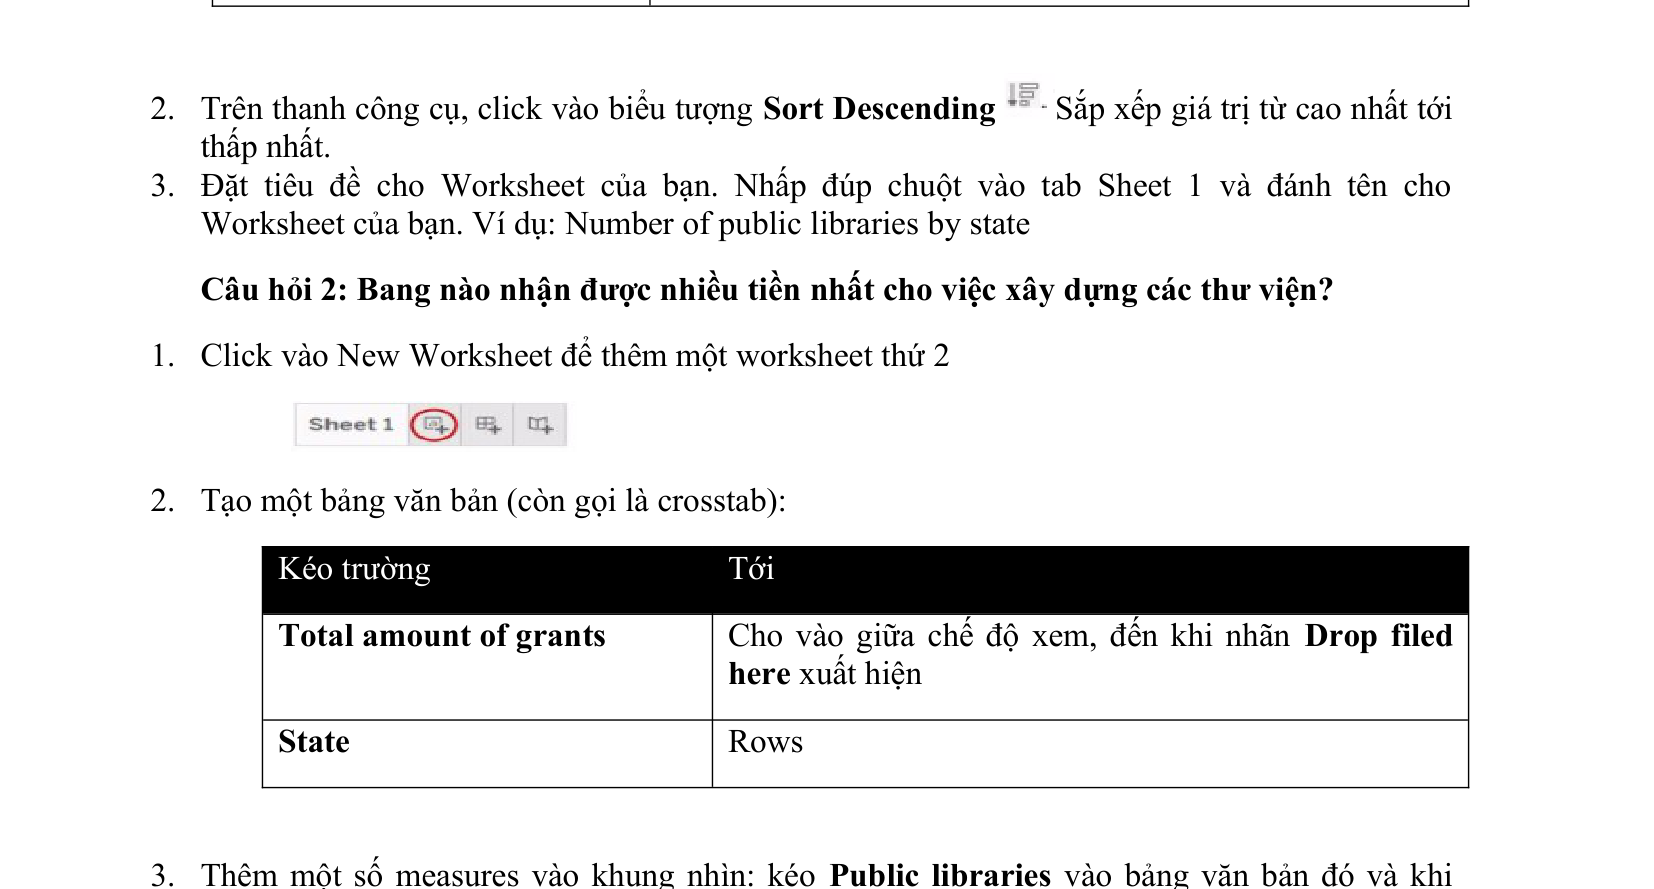
\includegraphics[width=0.9\linewidth]{images/text_table_crosstab.png}
\begin{figurecaptionmodern}
        \capfig{Text Table (Crosstab) --- Hướng dẫn tạo bảng chéo với việc kéo measure vào giữa view và Dimension vào Rows.}
        \label{fig:text_table}
    \end{figurecaptionmodern}
\end{figure}

% ===================================================================
\subsection{Maps --- Trực quan hóa dữ liệu địa lý}
% ===================================================================

\subsubsection{Khi nào dùng Maps?}

\noindent Khi dữ liệu chứa \textbf{thông tin địa lý} (Country, State, City, Postal Code), bản đồ là cách trực quan nhất để trả lời câu hỏi: \textit{``Khu vực nào có doanh thu cao nhất? Vùng nào có nhiều khách hàng?''} Tableau tự nhận diện các field địa lý (qua icon \faIcon{globe} trong Data Pane) và tự động tạo bản đồ khi bạn sử dụng chúng.

\noindent Tableau hỗ trợ \textbf{2 loại bản đồ chính}:

\begin{center}
\renewcommand{\arraystretch}{1.4}
\begin{tabularx}{\linewidth}{l X X}
\toprule
\textbf{Loại} & \textbf{Mô tả} & \textbf{Khi nào dùng} \\
\midrule
\textbf{Symbol Map} & Mỗi vị trí được đánh dấu bằng \textbf{điểm tròn} --- kích thước và màu thay đổi theo Measure & Dữ liệu theo điểm (thành phố, cửa hàng, khách hàng) \\
\textbf{Filled Map} & Tô màu toàn bộ \textbf{vùng} (quốc gia, bang) theo giá trị Measure & So sánh vùng/khu vực, choropleth map \\
\bottomrule
\end{tabularx}
\end{center}

\subsubsection{Cách tạo Symbol Map}

\noindent \textbf{Bước 1:} Double-click vào field \textbf{\texttt{State}} (hoặc bất kỳ Geographic field) trong Data Pane. Tableau tự động tạo bản đồ với các điểm đánh dấu trên từng State. Phía sau, Tableau sử dụng \textbf{Latitude (generated)} và \textbf{Longitude (generated)} để định vị.

\noindent \textbf{Bước 2:} Kéo \textbf{\texttt{Sales}} vào ô \textbf{Size} trong Marks card. Giờ các điểm có kích thước khác nhau --- điểm lớn = doanh thu cao.

\noindent \textbf{Bước 3:} Kéo \textbf{\texttt{Profit}} vào ô \textbf{Color} trong Marks card. Các điểm được tô màu từ đỏ (âm / lỗ) đến xanh (dương / lãi). Lúc này bản đồ cho thấy cả \textbf{quy mô} (kích thước) và \textbf{hiệu suất} (màu) của từng State.

\subsubsection{Cách tạo Filled Map}

\noindent \textbf{Bước 1:} Double-click vào field \textbf{\texttt{State}} để tạo bản đồ cơ bản.

\noindent \textbf{Bước 2:} Trong \textbf{Marks card}, chuyển dropdown \textbf{Mark Type} từ \textbf{Automatic} sang \textbf{Filled Map} (hoặc \textbf{Map}). Toàn bộ vùng của mỗi State được tô màu.

\noindent \textbf{Bước 3:} Kéo \textbf{\texttt{Sales}} vào \textbf{Color}. Các State có doanh thu cao sẽ có màu đậm hơn.

\begin{notebox}
\textbf{Xử lý vị trí không nhận được.} Đôi khi Tableau không nhận ra một số địa danh --- góc dưới bên phải xuất hiện thông báo \textbf{``X unknown''}. Nhấp vào đó $\rightarrow$ \textbf{Edit Locations} $\rightarrow$ chỉnh sửa bằng tay (gán đúng tên quốc gia, bang). Với dataset Superstore (có field Country, State, City), Tableau nhận diện gần như 100\% chính xác.
\end{notebox}

\begin{guidelinebox}{Symbol Map vs Filled Map: khi nào dùng cái nào?}
\renewcommand{\arraystretch}{1.3}
\begin{tabularx}{\linewidth}{l X X}
\toprule
\textbf{Tiêu chí} & \textbf{Symbol Map} & \textbf{Filled Map} \\
\midrule
Phù hợp & Dữ liệu theo điểm (cửa hàng, khách hàng) & Dữ liệu theo vùng (quốc gia, bang) \\
Nhiều Measure & Kích thước + Màu = 2 Measure & Chỉ Màu = 1 Measure \\
Vùng nhỏ & Vẫn thấy rõ (điểm tròn) & Dễ bị lấp bởi vùng lớn \\
\bottomrule
\end{tabularx}
\end{guidelinebox}

% ===================================================================
\subsection{Treemap \& Packed Bubbles --- Tỷ lệ phần trong tổng thể}
% ===================================================================

\subsubsection{Khi nào dùng Treemap / Packed Bubbles?}

\noindent Treemap và Packed Bubbles đều trả lời câu hỏi: \textit{``Phần nào chiếm tỷ trọng lớn nhất trong tổng thể?''} Thay vì dùng chiều dài thanh (Bar Chart), chúng dùng \textbf{kích thước hình} để thể hiện tỷ lệ --- hình lớn = giá trị lớn.

\begin{center}
\renewcommand{\arraystretch}{1.4}
\begin{tabularx}{\linewidth}{l X X}
\toprule
\textbf{Loại} & \textbf{Hình dạng} & \textbf{Đặc điểm} \\
\midrule
\textbf{Treemap} & Hình chữ nhật lồng nhau & Sử dụng không gian hiệu quả, hỗ trợ phân cấp (Category $\rightarrow$ Sub-Category) \\
\textbf{Packed Bubbles} & Hình tròn xếp sát nhau & Trực quan, dễ nhìn, phù hợp trình bày nhưng kém chính xác khi so sánh \\
\bottomrule
\end{tabularx}
\end{center}

\subsubsection{Cách tạo Treemap}

\noindent \textbf{Bước 1:} Kéo \textbf{\texttt{Sub-Category}} vào ô \textbf{Detail} (hoặc \textbf{Label}) trong Marks card. Mỗi Sub-Category sẽ trở thành một hình chữ nhật.

\noindent \textbf{Bước 2:} Kéo \textbf{\texttt{Sales}} vào ô \textbf{Size} trong Marks card. Kích thước mỗi ô tỷ lệ với doanh thu --- ô lớn nhất là Sub-Category có doanh thu cao nhất.

\noindent \textbf{Bước 3:} Kéo \textbf{\texttt{Category}} vào ô \textbf{Color} trong Marks card. Mỗi Category được gán một màu riêng, giúp phân biệt nhóm. Nếu chưa tự động hiển thị Treemap, chuyển \textbf{Mark Type} sang \textbf{Square} hoặc dùng \textbf{Show Me $\rightarrow$ Treemap}.

\noindent \textbf{Bước 4 (tùy chọn):} Kéo \textbf{\texttt{Sales}} vào \textbf{Label} để hiển thị giá trị trên mỗi ô.

\subsubsection{Cách tạo Packed Bubbles}

\noindent Tương tự Treemap nhưng thay \textbf{Mark Type = Circle}:

\begin{enumerate}[nosep]
    \item Kéo \textbf{\texttt{Sub-Category}} vào \textbf{Detail} --- mỗi giá trị thành một bọt.
    \item Kéo \textbf{\texttt{Sales}} vào \textbf{Size} --- bọt lớn = doanh thu cao.
    \item Kéo \textbf{\texttt{Category}} vào \textbf{Color} --- phân màu theo nhóm.
    \item Chuyển \textbf{Mark Type} sang \textbf{Circle} (hoặc dùng \textbf{Show Me $\rightarrow$ Packed Bubbles}).
    \item (Tùy chọn) Kéo \textbf{\texttt{Sub-Category}} vào \textbf{Label} để hiển thị tên trên mỗi bọt.
\end{enumerate}

\begin{guidelinebox}{Treemap vs Bar Chart: khi nào chọn Treemap?}
Bar Chart vẫn \textbf{chính xác hơn} khi so sánh giá trị (mắt người đánh giá chiều dài tốt hơn diện tích). Treemap nổi bật khi:
\begin{itemize}[nosep]
    \item Dữ liệu có \textbf{phân cấp} (Category $\rightarrow$ Sub-Category $\rightarrow$ Product) --- Treemap thể hiện tự nhiên bằng ô lồng nhau
    \item Có \textbf{rất nhiều danh mục} (20--50+) --- Bar Chart với 50 cột sẽ rất dài, Treemap gọn gàng hơn
    \item Muốn nhấn mạnh \textbf{tỷ trọng} hơn là giá trị tuyệt đối
\end{itemize}
\end{guidelinebox}

% ===================================================================
\subsection{Tổng kết --- Chọn chart phù hợp trong 10 giây}
% ===================================================================

\noindent Sau khi đã quen với cả 10 loại biểu đồ, chúng ta có thể rút gọn quy trình chọn chart thành một flow đơn giản: nhìn vào \textbf{kiểu dữ liệu} và \textbf{mục đích phân tích} để quyết định ngay.

\begin{center}
\renewcommand{\arraystretch}{1.3}
\small
\begin{tabularx}{\linewidth}{l X l l}
\toprule
\textbf{Loại biểu đồ} & \textbf{Câu hỏi trả lời} & \textbf{Trục X cần gì} & \textbf{Trục Y cần gì} \\
\midrule
\textbf{Bar Chart} & Cái nào lớn hơn/nhỏ hơn? & Dimension & Measure \\
\textbf{Line Chart} & Xu hướng thay đổi thế nào? & Date (liên tục) & Measure \\
\textbf{Area Chart} & Khối lượng + tỷ trọng theo thời gian? & Date (liên tục) & Measure \\
\textbf{Scatter Plot} & Hai chỉ số liên quan thế nào? & Measure & Measure \\
\textbf{Histogram} & Dữ liệu phân bố như thế nào? & Bins (liên tục) & Count \\
\textbf{Box Plot} & Phân phối giữa các nhóm? & Dimension & Measure (disagg.) \\
\textbf{Text Table} & Con số chính xác? Pattern? & Dimension & Dimension \\
\textbf{Maps} & Vùng nào nổi bật? & Geographic & \textit{(tự động)} \\
\textbf{Treemap} & Tỷ lệ phần trong tổng thể? & \textit{(không dùng shelf)} & \textit{(Size + Color)} \\
\bottomrule
\end{tabularx}
\end{center}

\noindent \textbf{Bộ câu hỏi quyết định nhanh:}

\begin{enumerate}[nosep]
    \item Dữ liệu có \textbf{địa lý} không? $\rightarrow$ \textbf{Maps}
    \item Trục X có phải \textbf{thời gian} không?
    \begin{itemize}[nosep]
        \item Muốn xem xu hướng? $\rightarrow$ \textbf{Line Chart}
        \item Muốn xem khối lượng/tỷ trọng? $\rightarrow$ \textbf{Area Chart}
    \end{itemize}
    \item Cả 2 trục đều là \textbf{số}? $\rightarrow$ \textbf{Scatter Plot}
    \item Muốn xem \textbf{phân phối}?
    \begin{itemize}[nosep]
        \item 1 nhóm? $\rightarrow$ \textbf{Histogram}
        \item Nhiều nhóm so sánh? $\rightarrow$ \textbf{Box Plot}
    \end{itemize}
    \item Cần \textbf{con số chính xác}? $\rightarrow$ \textbf{Text Table} (thêm màu = \textbf{Highlight Table / Heat Map})
    \item Muốn xem \textbf{tỷ trọng} với nhiều danh mục? $\rightarrow$ \textbf{Treemap / Packed Bubbles}
    \item Còn lại (so sánh danh mục) $\rightarrow$ \textbf{Bar Chart}
\end{enumerate}

\begin{notebox}
\textbf{Cạm bẫy phổ biến --- Line Chart cho dữ liệu phân loại.} Một sai lầm rất thường gặp là dùng Line Chart để so sánh các danh mục (ví dụ: 5 khu vực địa lý). Đường nối giữa ``North'' và ``East'' về mặt kỹ thuật được vẽ được, nhưng không có ý nghĩa thống kê --- ``North'' và ``East'' không có quan hệ liên tục. Bar Chart mới là lựa chọn đúng trong trường hợp này.
\end{notebox}

\noindent \textbf{Tóm tắt:} Sử dụng bảng và bộ câu hỏi ở trên để chọn chart phù hợp cho mọi tình huống phân tích. Khi không chắc chắn, hãy thử nhiều loại và để câu hỏi kinh doanh dẫn dắt lựa chọn.

\vspace{1em}
\noindent \textit{Kết thúc phần Basic Charts. Tiếp theo: Bài tập tổng hợp.}

% Reference ------------------------------------------------------------------
\newpage
\section{Tài liệu tham khảo}
\label{section:references}
\nocite{*}
\vspace{-3.2em}
\printbibliography

% Appendix -------------------------------------------------------------------
\newpage
\begin{appendices}

\section{Nội dung Phụ lục}

\begin{enumerate}
    \item \textbf{Datasets:} Các file dataset được đề cập trong bài có thể được tải tại \href{https://aivietnam.edu.vn/}{đây}.
    \item \textbf{Hint:} Các file code gợi ý có thể được tải tại \href{https://aivietnam.edu.vn/}{đây}.
    \item \textbf{Solution:} Các file code cài đặt hoàn chỉnh và phần trả lời nội dung trắc nghiệm có thể được tải tại \href{https://aivietnam.edu.vn/}{đây}.
\end{enumerate}

\end{appendices}
\end{document}
